\documentclass[11pt]{beamer}


\usetheme{metropolis}
\metroset{everytitleformat = regular,progressbar=foot} %settings
\mode<presentation>
%\usecolortheme{dove} %dove
% albatross, beaver, beetle, crane, default, dolphin, dove, orchid, rose, seagull, seahorse, whale, wolverine
%dont use  fly, lily,
%http://mirror.ox.ac.uk/sites/ctan.org/macros/latex/contrib/beamer/doc/beameruserguide.pdf
\setbeamercolor{title separator}{fg = UniBlue}
\setbeamercolor{frametitle}{fg = deepBlue, bg=aBlue!70}

\usepackage{booktabs}
\usepackage[scale=2]{ccicons}

\usepackage{pgfplots}
\usepgfplotslibrary{dateplot}


%coords are in relation to lower right corner
%\logo{\pgfputat{\pgfxy(0,6}{\pgfbox[right,top]{
\includegraphics[width=2.5cm]{logo.png}}}}

\usepackage{tikz}
\addtobeamertemplate{frametitle}{}{%
\begin{tikzpicture}[remember picture,overlay]
\node[anchor=north east,yshift=2pt] at (current page.north east) {
\includegraphics[height=0.8cm]{logo.png}};
\end{tikzpicture}}

%My std preamble for the docs
%\selectlanguage{british}%
\usepackage[british]{babel}
\usepackage{microtype} %better text
\IfFileExists{lmodern.sty}{\usepackage{lmodern}}{} %type 1 vector font
%
\usepackage{lettrine}
\usepackage{listings} %Add list support
\usepackage{colortbl} %colors in TABLES
%\usepackage{tikz,amsmath, amssymb,bm,color}
\usepackage{nicefrac}
\usepackage{lastpage} %get last page

%COLORS
\usepackage{color}
\definecolor{lightgray}{gray}{0.8} %for colortbl
\definecolor{UniBlue}{RGB}{83,121,170}
\definecolor{deepBlue}{HTML}{000066}
\definecolor{blueBgd}{HTML}{99C8FF}
\definecolor{aBlue}{HTML}{1879F7}

%%%%%%%%%%%%%%%%%%%%%%%%%%%%%%%%%%%%%%%%%%%%%%%%%%%%%%%%%%%%%%%%%%
%FOOTNOTES
%nice look after http://www.dedoimedo.com


%%%%%%%%%%%%%%%%%%%%%%%%%%%%%%%%%%%%%%%%%%%%%%%%%%%%%%%%%%%%%%%%%%%
%TABLE SETTINGS
\usepackage{colortbl} %colors in table
\usepackage{rotating} %rotatins within tables
\usepackage{multirow}
\renewcommand{\arraystretch}{1.2} %add padding/spacing
%\usepackage{adjustbox}%rotating and fitting into page
%

\usepackage{booktabs} % To thicken table lines
%define thickness of table lines
\let\mytoprule\toprule
\renewcommand{\toprule}{\mytoprule[0.20em]}
\let\mytoprule\bottomrule
\renewcommand{\bottomrule}{\mytoprule[0.20em]}
\let\mytoprule\midrule
\renewcommand{\midrule}{\mytoprule[0.08em]}

\usepackage{spreadtab} % for simple calculations

%vertically and horizontally centered multicolumn cells with a fixed width. M{width}
%\newcolumntype{M}[1]{>{\centering\hspace{0pt}}m{#1}}
% each spanned cell has the same width. S{width of multicolumn cell}{number of spanned columns}
%\newcolumntype{S}[2]{>{\centering\hspace{0pt}}m{(#1+(2\tabcolsep+\arrayrulewidth)*(1-#2))/#2}}

%%%%%%%%%%%%%%%%%%%%%%%%%%%%%%%%%%%%%%%%%%%%%%%%%%%%%%%%%%%%%%%%%%%
%TikZ
\usepackage{tikz}

\colorlet{red}{red!50}
\colorlet{green}{green!50}
\colorlet{blue}{blue!50}
\definecolor{yellow}{HTML}{FFFF00}
\colorlet{yellow}{yellow!50}
\definecolor{fiolet}{HTML}{7030A0}
\colorlet{fiolet}{fiolet!50}
\colorlet{bgd_main}{black!50}
\colorlet{bgd}{bgd_main!75}
\colorlet{bgd2}{bgd_main!50}
\colorlet{bgd3}{bgd_main!25}
\colorlet{bgd4}{bgd_main!15}

\usetikzlibrary{shapes,arrows,calc,positioning}

%%%%%%%%%%%%%%%%%%%%%%%%%%%%%%%%%%%%%%%%%%%%%%%%%%%%%%%%%%%%%%%%%%%
% Footnotes in Figs
%\rule[raise-height]{width}{thickness}
\newcommand*{\FigFootnote}[1]{
\noindent \begin{flushleft}
\rule[0.2ex]{0.4\columnwidth}{0.5pt}
\par
\footnotesize
#1
\footnotesize
\end{flushleft}
}

%%%%%%%%%%%%%%%%%%%%%%%%%%%%%%%%%%%%%%%%%%%%%%%%%%%%%%%%%%%%%%%%%%%
%MATH, number display
%need to install siunitx, l3kernel,l3packages
\usepackage{siunitx} %this is for units display

\sisetup{per-mode=fraction, tight-spacing = true , fraction-function = \nicefrac, quotient-mode = fraction}% %nicefrac \tfrac
\sisetup{inter-unit-product = \ensuremath { { } \cdot { } } , exponent-product = \cdot }%
\sisetup{input-product=x , output-quotient =  \ensuremath { { } \times{}}} %for 1x2x3
%number grouping(3), std==true %\sisetup{group-digits = decimal} 
\sisetup{group-minimum-digits = 4} %start grouping from 4 digits, in 3 no groups
\sisetup{range-units = single,range-phrase = \,--\,} %2-3C not 2C-3C %, range-phrase = --
\sisetup{separate-uncertainty=true} %2+-1 not 2(1)
\sisetup{prefixes-as-symbols=true } % , scientific-notation = engineering false for 10^-9 ect ect , exp in multiple of 3
\sisetup{range-phrase = \,-\, } % , refo of ranges
%\sisetup{zero-decimal-to-integer, round-mode = places,round-precision = 3}
%\sisetup{add-arc-degree-zero=true , add-arc-minute-zero=true ,add-arc-second-zero=true} %for angle settings

%This is to auto convert ns,ms,us to 10^-xx s
\DeclareSIUnit[scientific-notation = engineering, prefixes-as-symbols=false]{\psec}{\pico\second}
\DeclareSIUnit[scientific-notation = engineering, prefixes-as-symbols=false]{\nsec}{\nano\second} 
\DeclareSIUnit[scientific-notation = engineering, prefixes-as-symbols=false]{\usec}{\micro\second}
\DeclareSIUnit[scientific-notation = engineering, prefixes-as-symbols=false]{\msec}{\milli\second} 

%...AND SOME UNITS
\DeclareSIUnit\dBm{dBm}
\DeclareSIUnit\ppm{ppm} %{\num{1e-6}}%{ppm}
\DeclareSIUnit\yr{yr} %{{361}\day}<-nice nice
\DeclareSIUnit\cy{cycle} %phase cycle
\DeclareSIUnit\epoch{epoch} %GPS/LL epoch
\DeclareSIUnit\inch{"} %inch 
\DeclareSIUnit\wk{week} %week
\DeclareSIUnit\hr{hrs} %hours
\DeclareSIUnit\min{minute} %hours
\DeclareSIUnit\mile{mi}
\DeclareSIUnit\Mcps{Mcps}
\DeclareSIUnit\bit{bit}
\DeclareSIUnit\chip{chip length}
%Other units
\newcommand*{\GBP}[1]{$\SI{#1}[\textsterling]{}$}


%%%%%SHORTHANDS (Standard Sentences)
%\newcommand*{\Myrange}[3]{$\textrm{\SIrange{#1}{#2}{#3}}$}


%how much work per week
\newcommand*{\wkWrk}[1]{$\SI{#1}{\hr\per\wk}$}

%references
\newcommand*{\tabref}[1]{shown in table \ref{#1} on page \pageref{#1}\xspace}
\newcommand*{\vref}[1]{\ref{#1} on page \pageref{#1}\xspace}


%\renewcommand{\baselinestretch}{1.2} %line spacing
%{\setstretch{1.0}\color{blue} text bla bla } for section strech
\renewcommand{\footnotesize}{\scriptsize}
%\usepackage[demo]{graphicx}
\usepackage[font={small,it}]{caption}
\usepackage{subcaption}

%%%%%%%%%%%%%%%%%%%%%%%%%%%%%%%%%%%%%%%%%%%%%%%%%%%%%%%%%%%%%%%%%%%%%%%%%%%%%%

%\usepackage{lipsum} % for dummy text only

%Grey text
%\definecolor{shadecolor}{RGB}{190,190,190}
%\textcolor{shadecolor}{	\item[Ogaja\_Matlab.7z] Matlab script. To be placed on-line after week2.}


\title[TEQC MP]{Example of TEQC mulitpah results \\}
\author{LKB}
\institute{NGI}
\date{\today}

\begin{document}
	
	\begin{frame}
		\titlepage
	\end{frame}
	
	% Uncomment these lines for an automatically generated outline.
	%\begin{frame}{Outline}
	%  \tableofcontents
	%\end{frame}
	
\section{Introduction}
	
	\begin{frame}{Introductory notes}
		TEQC tutorial can be found at:\\
		\url{http://www.unavco.org/software/data-processing/TEQC/doc/UNAVCO_TEQC_Tutorial.pdf}\\
		TEQC website is at:\\
		\url{http://www.unavco.org/software/data-processing/TEQC/TEQC.html}\\
		\medskip
		TEQC can be downloaded from:\\
		\url{http://www.unavco.org/software/data-processing/TEQC/development/TEQC_mingw_64.zip} (x64 - 64 bit Windows)\\
		\url{http://www.unavco.org/software/data-processing/TEQC/development/TEQC_mingw_32.zip} (32 bit Windows)\\

		
	\end{frame}
	
	\begin{frame}{Support files}
		Following files can be found at H24VLP Moodle website (\url{http://moodle.nottingham.ac.uk/course/view.php?id=26398}):
		\begin{description}
			\item[TEQC\_intro.pdf] TEQC introductory document by Sean Ince;
			\item[MP\_TEQC.pdf] This presentation;
			\item[extractRinex4Msc.bat] Script (batch file) for RINEX extraction and TEQC QC analysis required for the practical;
			\item[extractMPdata.bat] Script to convert COMPACT2 format to csv file readable by Excel. See following slide for details.
			\item[ExtractSNR.py] Python script, part of extractMPdata.bat;
			\item[2006\_Ogaja.pdf] A paper discussing multipath analysis' in Matlab using TEQC QC output;
			\item[Matlab.zip] Matlab script, discussed in the paper above. Use \textit{main.m} to run it.
		\end{description}
		
	\end{frame}	


	\begin{frame}[allowframebreaks]{How to use my script}
		To use \textit{extractMPdata.bat}, script to convert COMPACT2 format to csv file readable by Excel, you need to:
		\begin{itemize}
			\item copy both extractMPdata.bat and ExtractSNR.py to same folder
			\item install python 2.7.x (\url{https://www.python.org/downloads/release/python-279/}
			\item install GPSToolkit (\url{(http://www.gpstk.org})
			\item add GPSToolkit to your PATH. 
				\begin{itemize}
					\item PATH will be under User variables
					\item append \path{;PATH\TO\GPSToolkit\bin} the end of the PATH variable.
					\item Go to COMPUTER$\rightarrow$PROPERTIES$\rightarrow$Advanced Properties$\rightarrow$Environmental Variable
					\item \textbf{DON'T OVERWRITE ORIGINAL PATH variable !!!}
				\end{itemize}
			\item run extractMPdata.bat in the same folder as TEQC QC output
		\end{itemize}
		
	\end{frame}	
	
	\begin{frame}{Workflow}
		In order to obtain multipath characteristics please follow those steps:
		
		\begin{itemize}
			\item Convert data to RINEX using TEQC (see my batch file or Sean's introduction);
			\item {Extract QC characteristics  (TEQC +qc obs file.15o or see my batch file )};
			\item Examine mp1 and mp2 files (using my python script for example);
			\item Plot results, for example in Excel;
			\item \textit{Use Ogaja Matlab script for additional analysis and visual representation of results;}
			\item \textbf{Analyse data and draw conclusions.}
		\end{itemize}

	\end{frame}

%changing settings for this area
{\sisetup{round-mode = places,round-precision = 3} 

\begin{frame}{Multipath Test}
	\begin{table}
		\centering
		\begin{minipage}[t]{\textwidth}%
			\resizebox{\columnwidth}{!}{%
				\begin{tabular}{lcccc} %{l|c|c|c|c}
					\toprule %\rowcolor{lightgray}
					ID & $E[m]$ & $N[m]$ & Ht Ort [m]\footnote{Geoid undulation is \num{48.523}m} & Notes \\
					\midrule
					JUB7 & \num{454729.5517} & \num{339338.9003} & \num{28.9802} & Open Space\\
					JUB8 & \num{454682.3444} & \num{339523.0937} & \num{27.8030} & Trees\\
					JUB9 & \num{454849.2113} & \num{339695.8759} & \num{29.9054} & MP for Group 1\\
					JUB10 & \num{454851.6669} & \num{339697.2905} & \num{29.8658} & MP for Group 2\\
				\end{tabular}%
			}
			\caption{OSGB coordinates for the Project 1}
		\end{minipage}
	\end{table}
	
\end{frame}


\section{Comparison examples}
	

\begin{frame}{Monday 12/01/15, MP1}
	\begin{figure}
		\centering
		\begin{subfigure}{.5\textwidth}
			\centering
			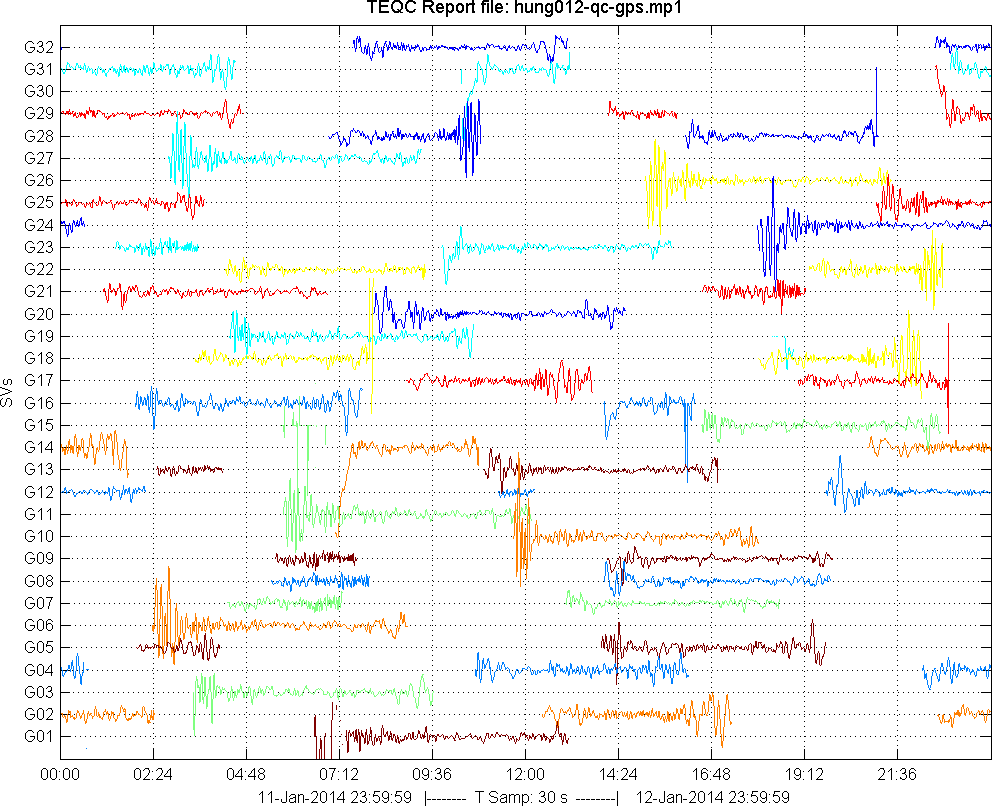
\includegraphics[width=\textwidth]{pic/hung012_qc_gps_mp1.png}
			\caption{HUNG, no MP}
			\label{fig:sub1}
		\end{subfigure}%
		\begin{subfigure}{.5\textwidth}
			\centering
			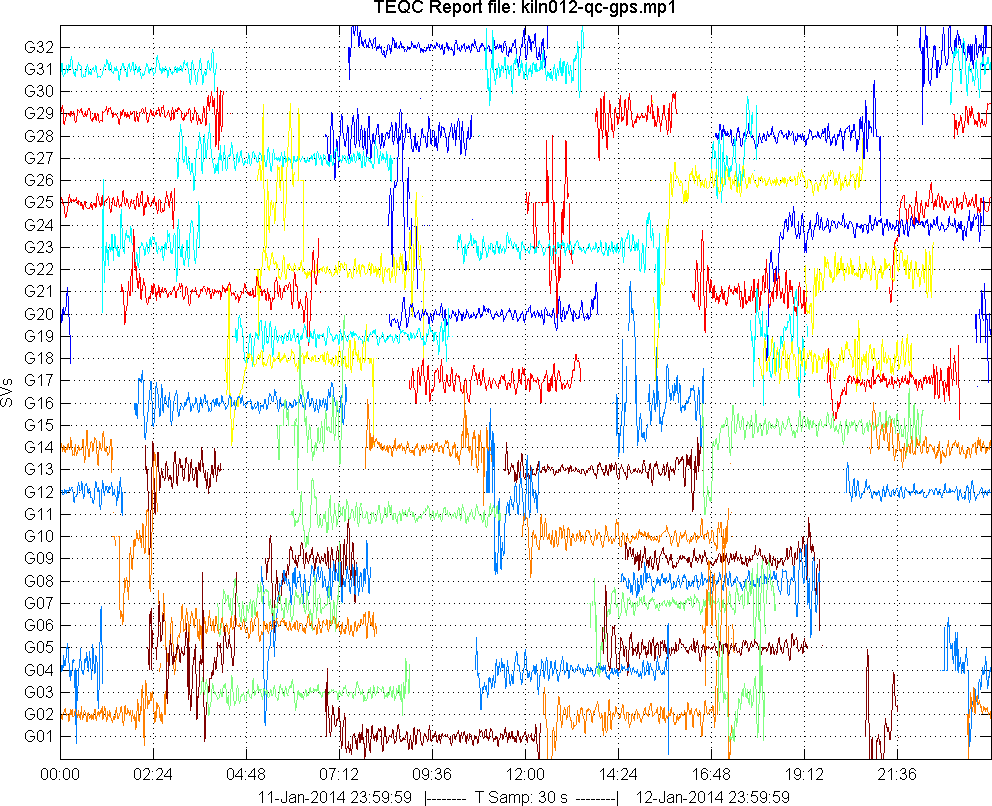
\includegraphics[width=\textwidth]{pic/kiln012_qc_gps_mp1.png}
			\caption{KILN, suspected MP}
			\label{fig:sub2}
		\end{subfigure}
		\caption{Comparison of TEQC MP1 outputs}
		% \label{fig:test}
	\end{figure}
\end{frame}

\begin{frame}{Monday 12/01/15, MP2}
	\begin{figure}
		\centering
		\begin{subfigure}{.5\textwidth}
			\centering
			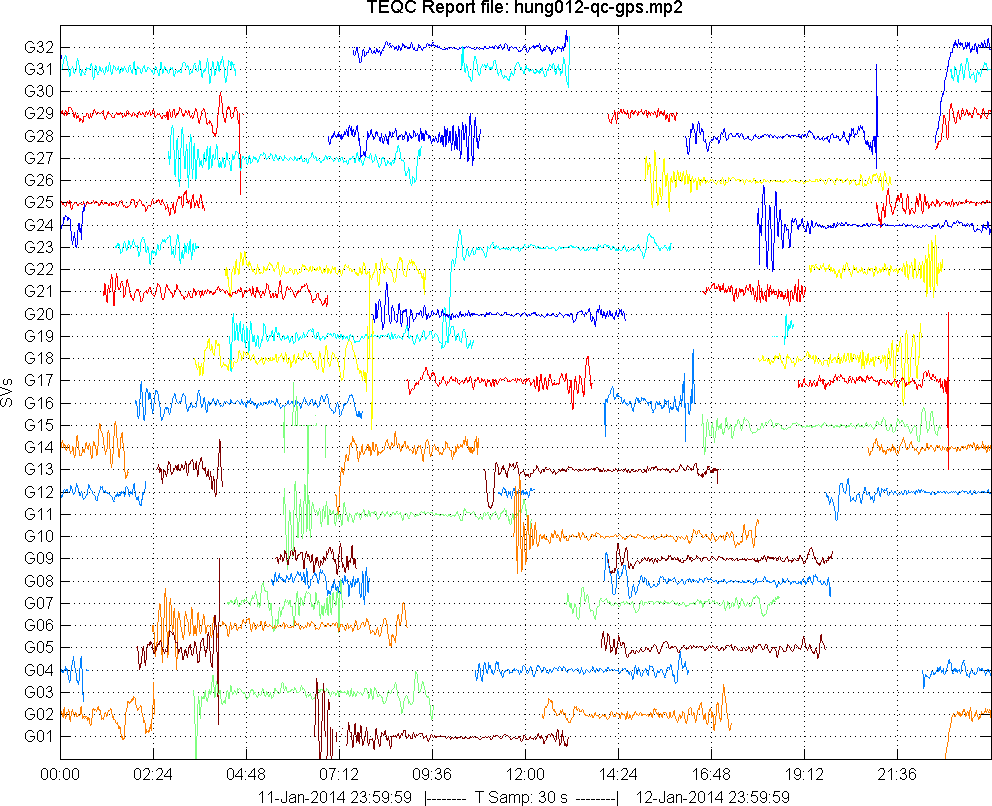
\includegraphics[width=\textwidth]{pic/hung012_qc_gps_mp2.png}
			\caption{HUNG, no MP}
			\label{fig:sub1}
		\end{subfigure}%
		\begin{subfigure}{.5\textwidth}
			\centering
			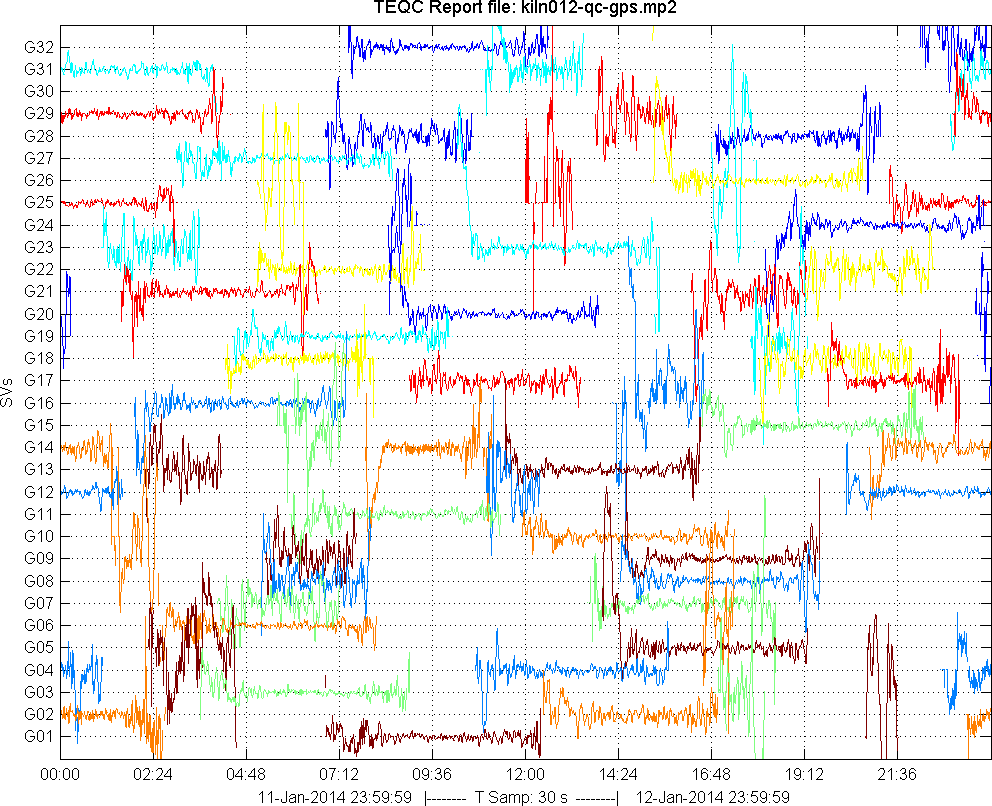
\includegraphics[width=\textwidth]{pic/kiln012_qc_gps_mp2.png}
			\caption{KILN, suspected MP}
			\label{fig:sub2}
		\end{subfigure}
		\caption{Comparison of TEQC MP2 outputs}
		% \label{fig:test}
	\end{figure}
\end{frame}

\begin{frame}{Tuesday 13/01/15, MP1}
	\begin{figure}
		\centering
		\begin{subfigure}{.5\textwidth}
			\centering
			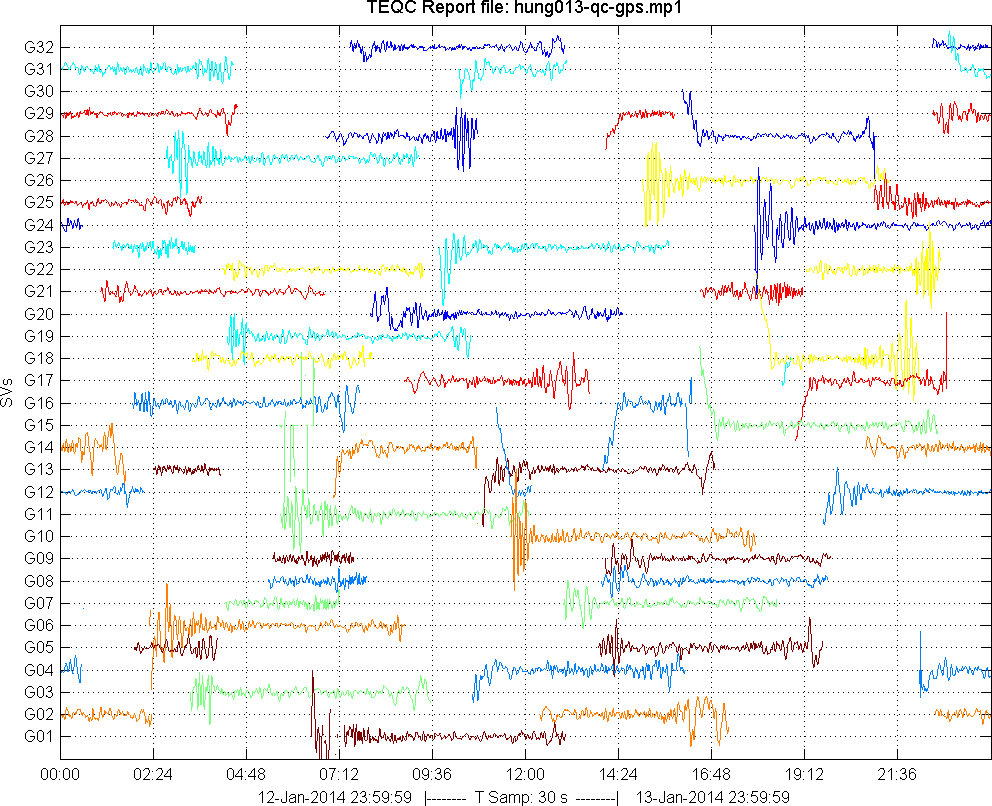
\includegraphics[width=\textwidth]{pic/hung013_qc_gps_mp1.png}
			\caption{HUNG, no MP}
			\label{fig:sub1}
		\end{subfigure}%
		\begin{subfigure}{.5\textwidth}
			\centering
			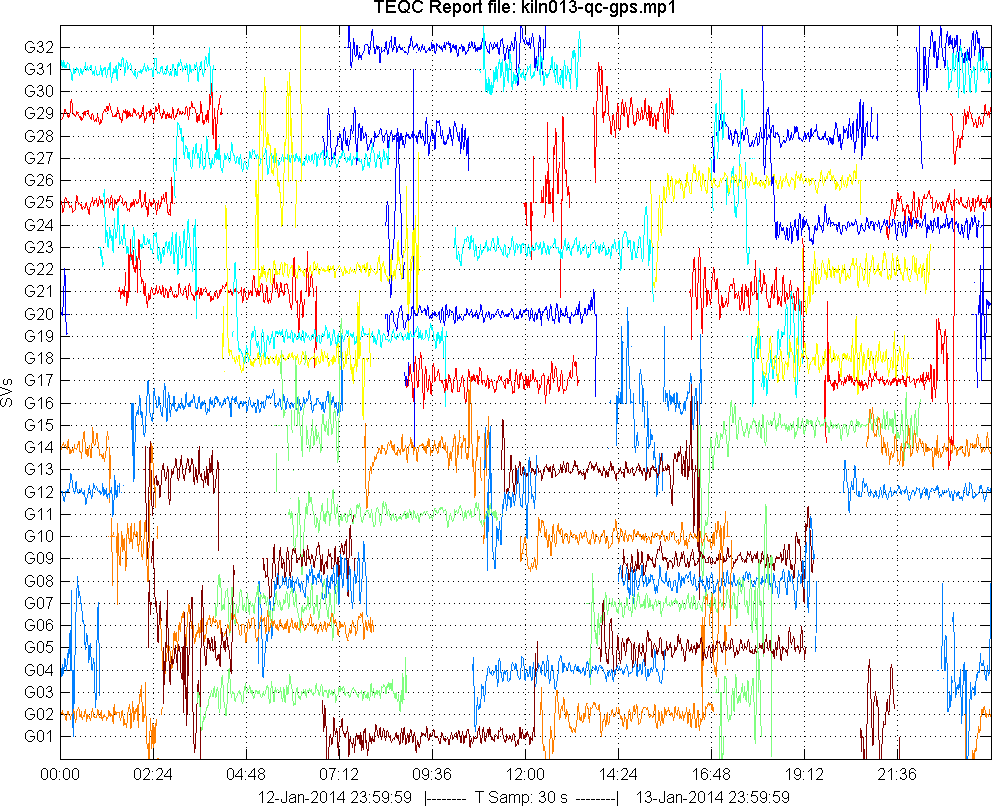
\includegraphics[width=\textwidth]{pic/kiln013_qc_gps_mp1.png}
			\caption{KILN, suspected MP}
			\label{fig:sub2}
		\end{subfigure}
		\caption{Comparison of TEQC MP1 outputs}
		% \label{fig:test}
	\end{figure}
\end{frame}

\begin{frame}{Tuesday 13/01/15, MP2}
	\begin{figure}
		\centering
		\begin{subfigure}{.5\textwidth}
			\centering
			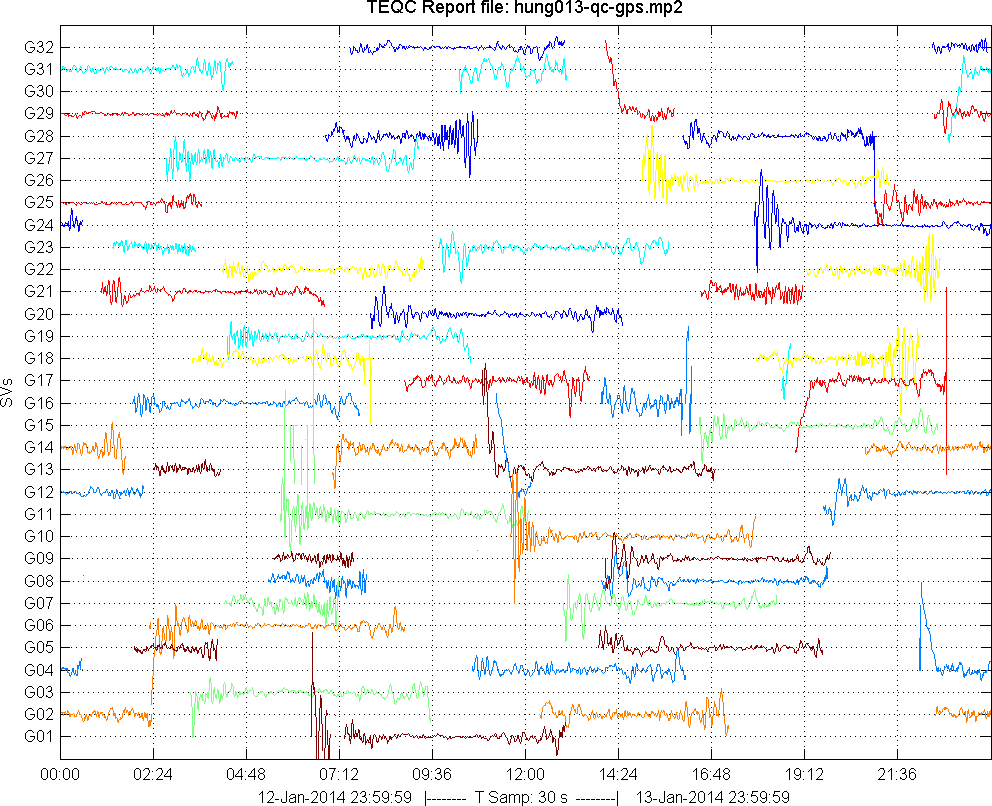
\includegraphics[width=\textwidth]{pic/hung013_qc_gps_mp2.png}
			\caption{HUNG, no MP}
			\label{fig:sub1}
		\end{subfigure}%
		\begin{subfigure}{.5\textwidth}
			\centering
			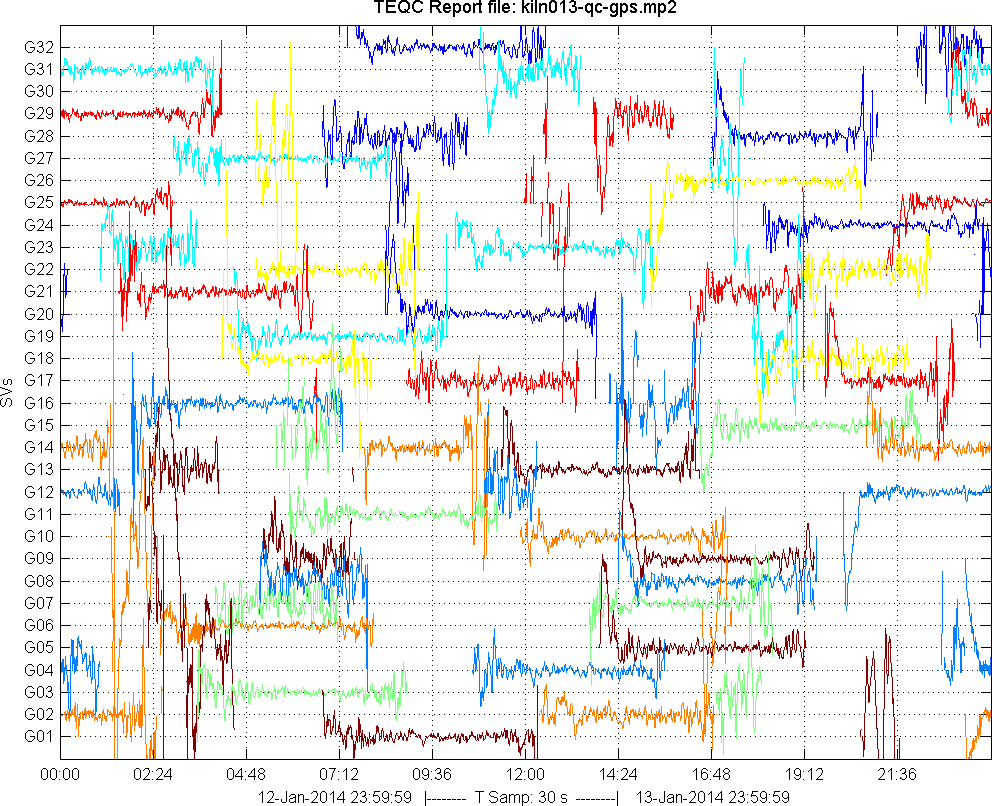
\includegraphics[width=\textwidth]{pic/kiln013_qc_gps_mp2.png}
			\caption{KILN, suspected MP}
			\label{fig:sub2}
		\end{subfigure}
		\caption{Comparison of TEQC MP2 outputs}
		% \label{fig:test}
	\end{figure}
\end{frame}

\begin{frame}{Wednesday 14/01/15, MP1}
	\begin{figure}
		\centering
		\begin{subfigure}{.5\textwidth}
			\centering
			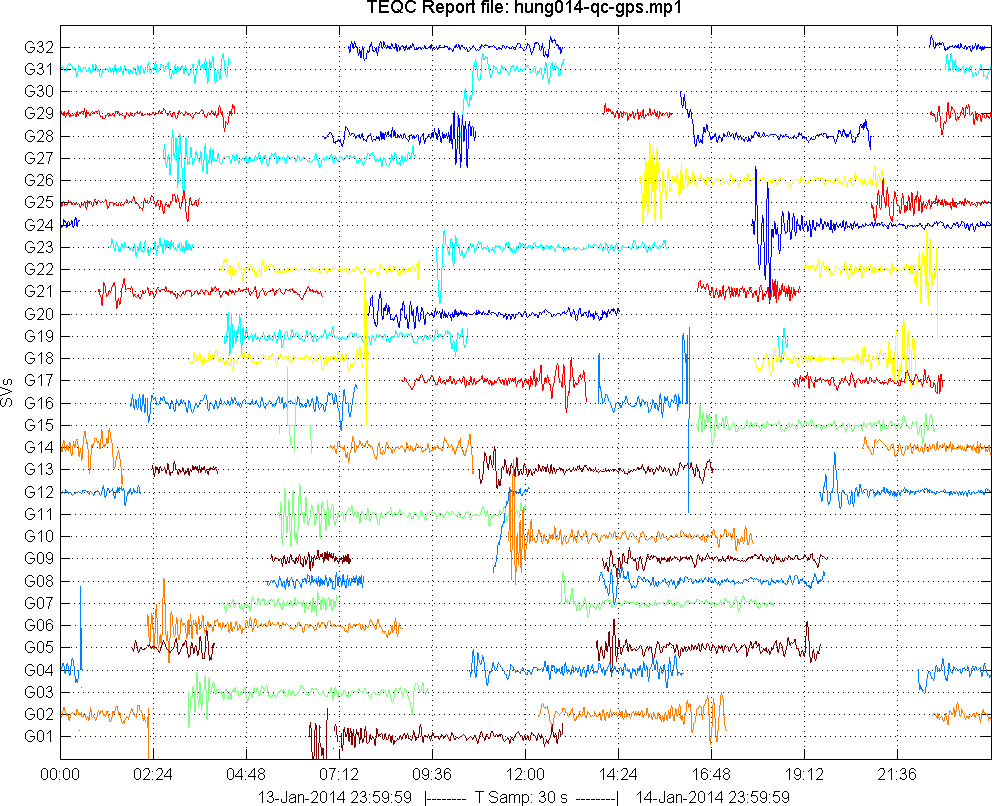
\includegraphics[width=\textwidth]{pic/hung014_qc_gps_mp1.png}
			\caption{HUNG, no MP}
			\label{fig:sub1}
		\end{subfigure}%
		\begin{subfigure}{.5\textwidth}
			\centering
			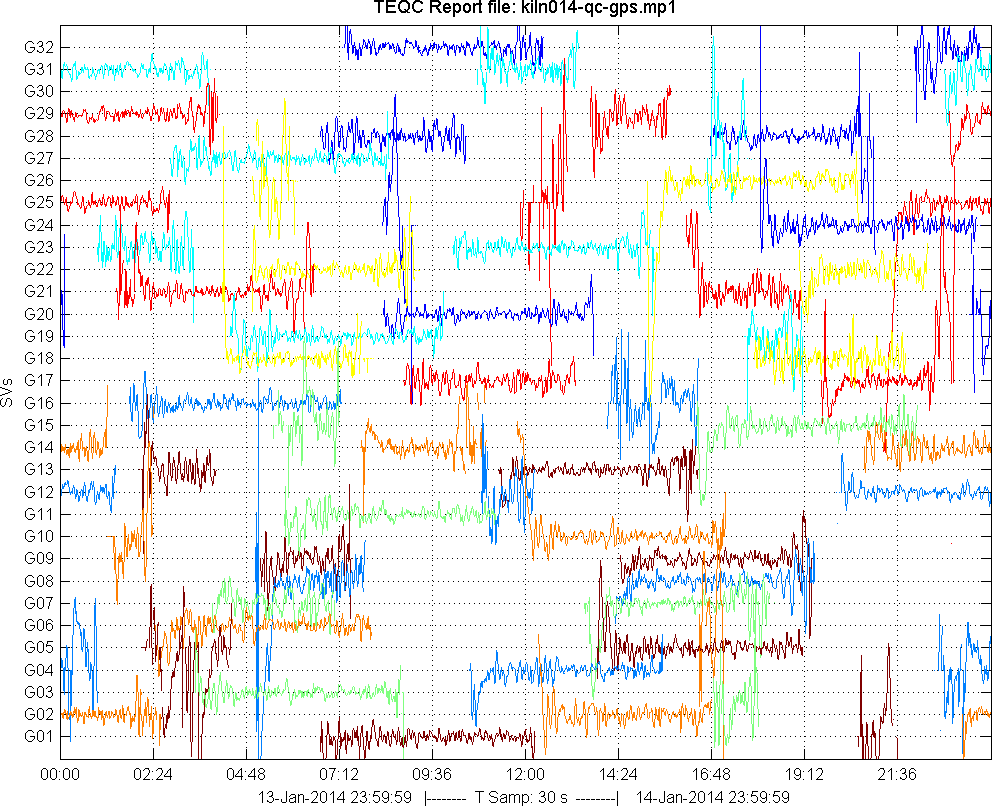
\includegraphics[width=\textwidth]{pic/kiln014_qc_gps_mp1.png}
			\caption{KILN, suspected MP}
			\label{fig:sub2}
		\end{subfigure}
		\caption{Comparison of TEQC MP1 outputs}
		% \label{fig:test}
	\end{figure}
\end{frame}

\begin{frame}{Wednesday 14/01/15, MP2}
	\begin{figure}
		\centering
		\begin{subfigure}{.5\textwidth}
			\centering
			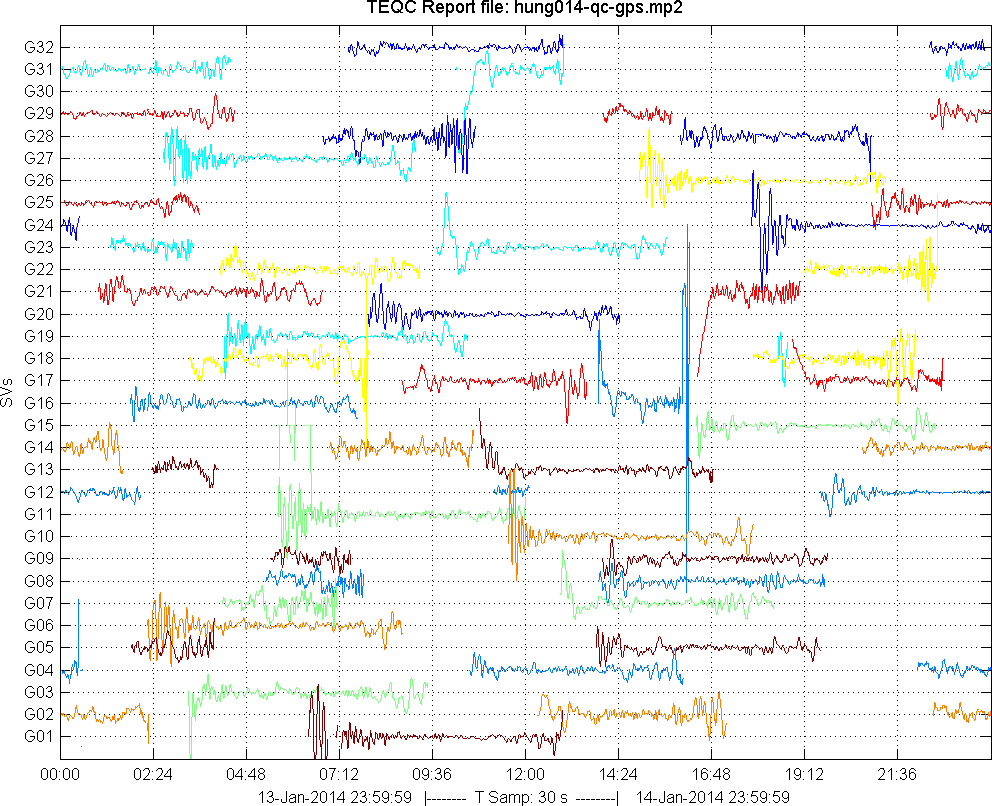
\includegraphics[width=\textwidth]{pic/hung014_qc_gps_mp2.png}
			\caption{HUNG, no MP}
			\label{fig:sub1}
		\end{subfigure}%
		\begin{subfigure}{.5\textwidth}
			\centering
			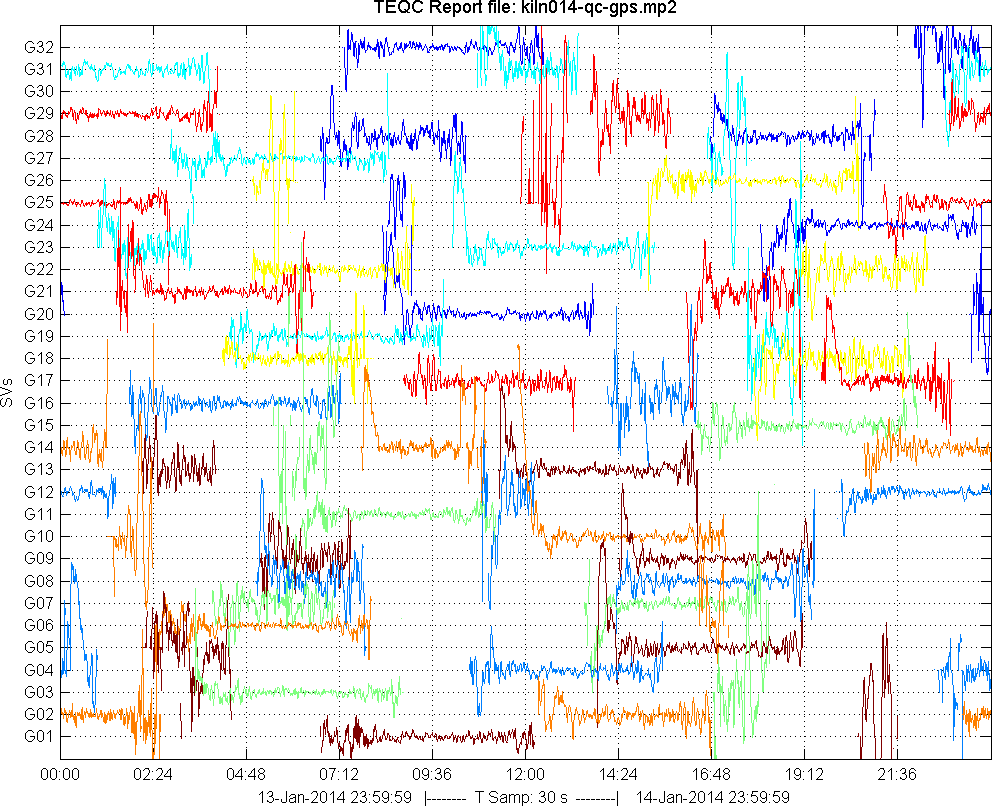
\includegraphics[width=\textwidth]{pic/kiln014_qc_gps_mp2.png}
			\caption{KILN, suspected MP}
			\label{fig:sub2}
		\end{subfigure}
		\caption{Comparison of TEQC MP2 outputs}
		% \label{fig:test}
	\end{figure}
\end{frame}

\begin{frame}{Thursday 15/01/15, MP1}
	\begin{figure}
		\centering
		\begin{subfigure}{.5\textwidth}
			\centering
			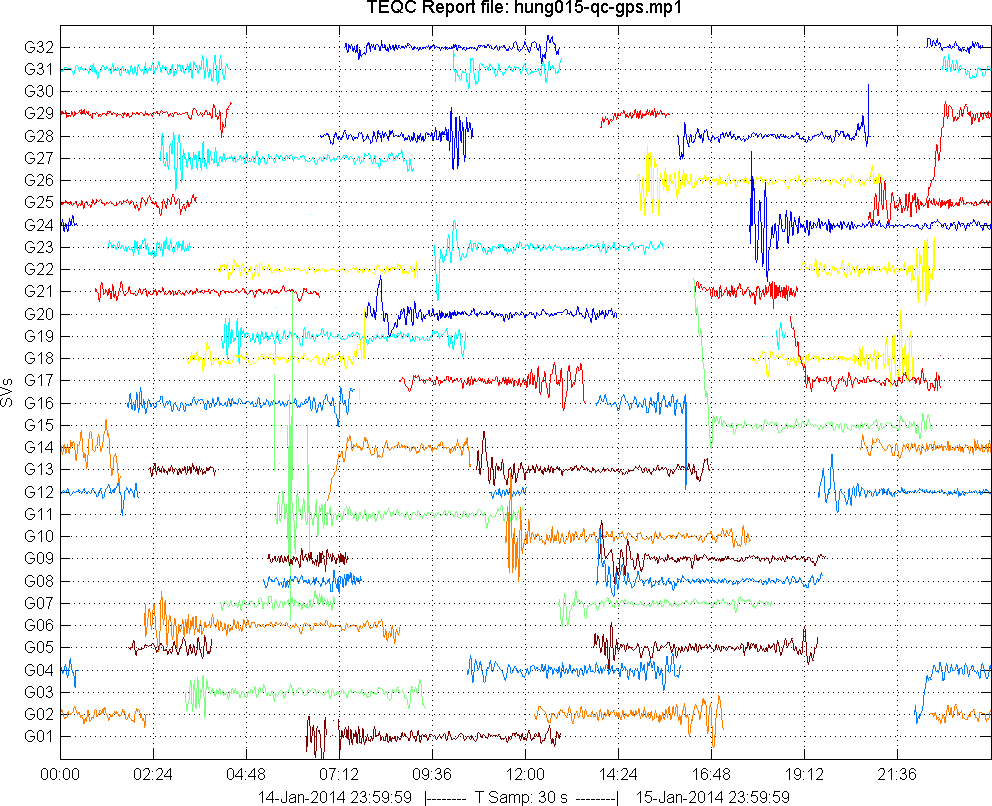
\includegraphics[width=\textwidth]{pic/hung015_qc_gps_mp1.png}
			\caption{HUNG, no MP}
			\label{fig:sub1}
		\end{subfigure}%
		\begin{subfigure}{.5\textwidth}
			\centering
			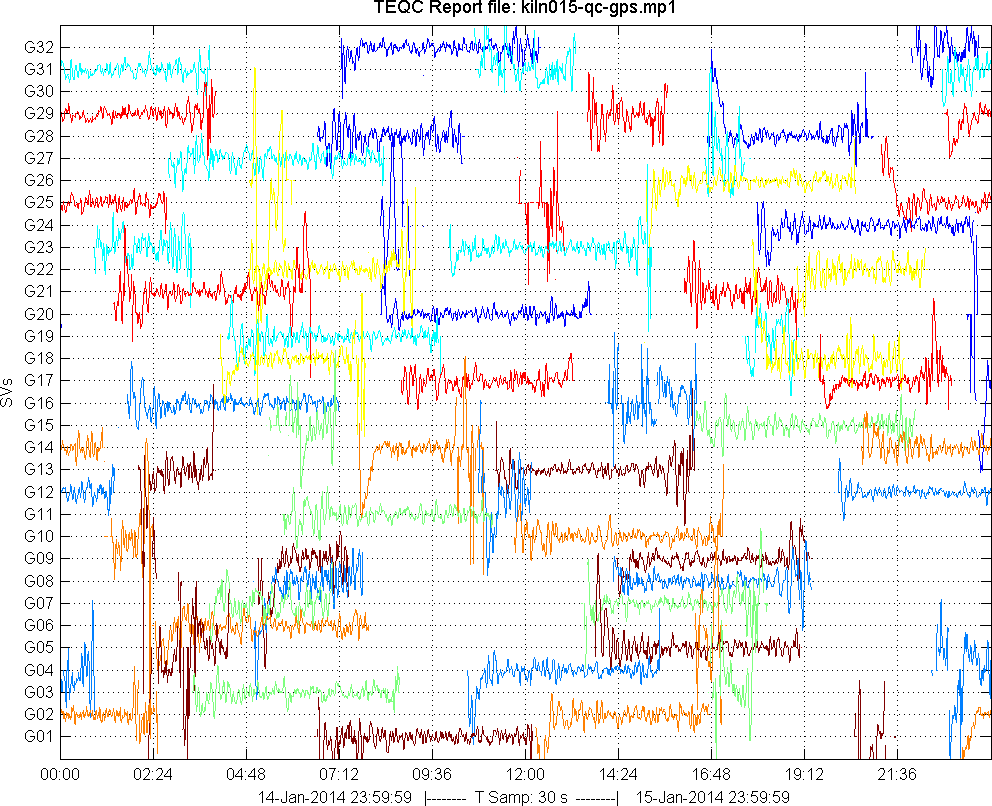
\includegraphics[width=\textwidth]{pic/kiln015_qc_gps_mp1.png}
			\caption{KILN, suspected MP}
			\label{fig:sub2}
		\end{subfigure}
		\caption{Comparison of TEQC MP1 outputs}
		% \label{fig:test}
	\end{figure}
\end{frame}

\begin{frame}{Thursday 15/01/15, MP2}
	\begin{figure}
		\centering
		\begin{subfigure}{.5\textwidth}
			\centering
			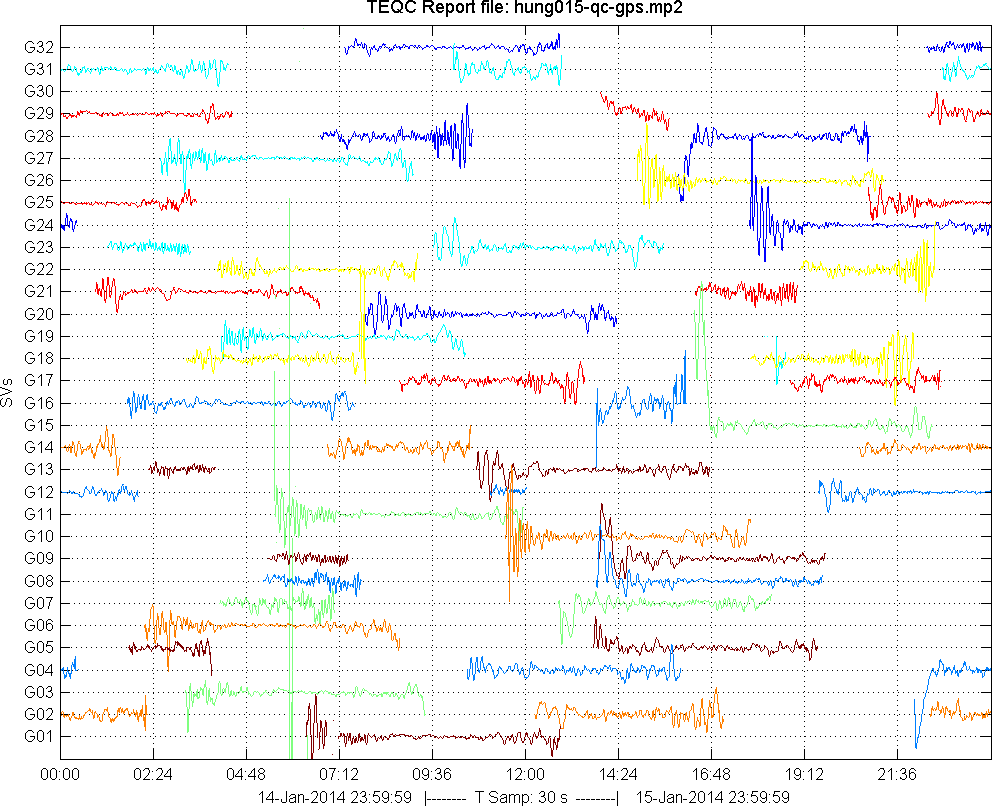
\includegraphics[width=\textwidth]{pic/hung015_qc_gps_mp2.png}
			\caption{HUNG, no MP}
			\label{fig:sub1}
		\end{subfigure}%
		\begin{subfigure}{.5\textwidth}
			\centering
			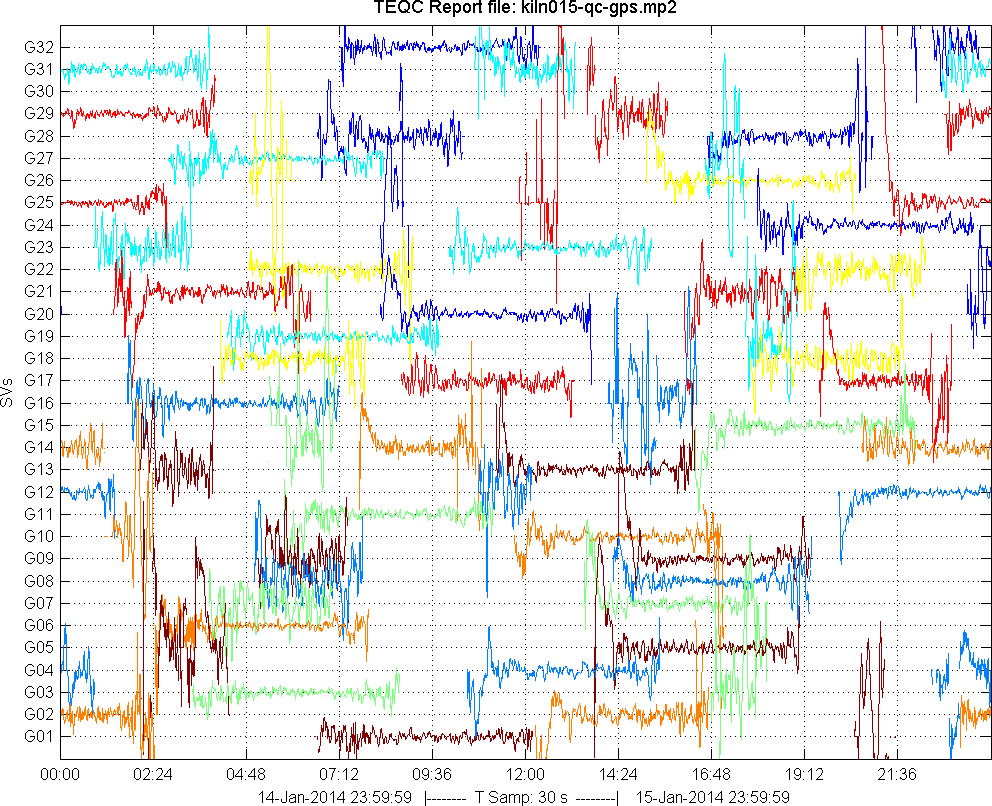
\includegraphics[width=\textwidth]{pic/kiln015_qc_gps_mp2.png}
			\caption{KILN, suspected MP}
			\label{fig:sub2}
		\end{subfigure}
		\caption{Comparison of TEQC MP2 outputs}
		% \label{fig:test}
	\end{figure}
\end{frame}

\begin{frame}{Friday 16/01/15, MP1}
	\begin{figure}
		\centering
		\begin{subfigure}{.5\textwidth}
			\centering
			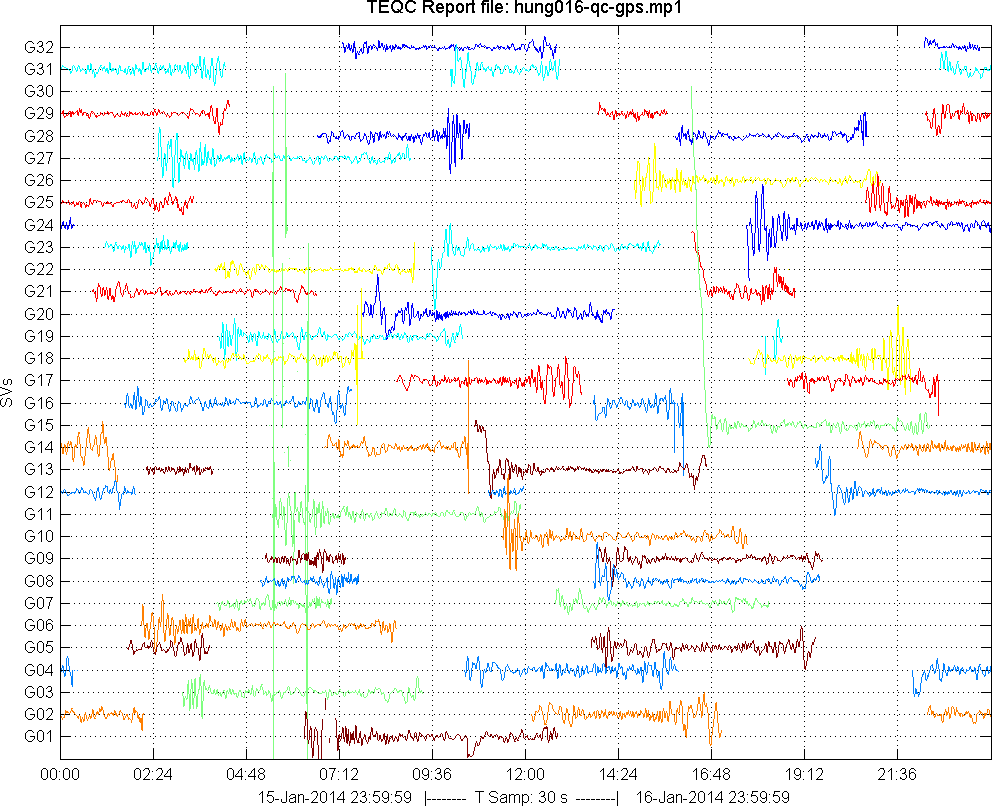
\includegraphics[width=\textwidth]{pic/hung016_qc_gps_mp1.png}
			\caption{HUNG, no MP}
			\label{fig:sub1}
		\end{subfigure}%
		\begin{subfigure}{.5\textwidth}
			\centering
			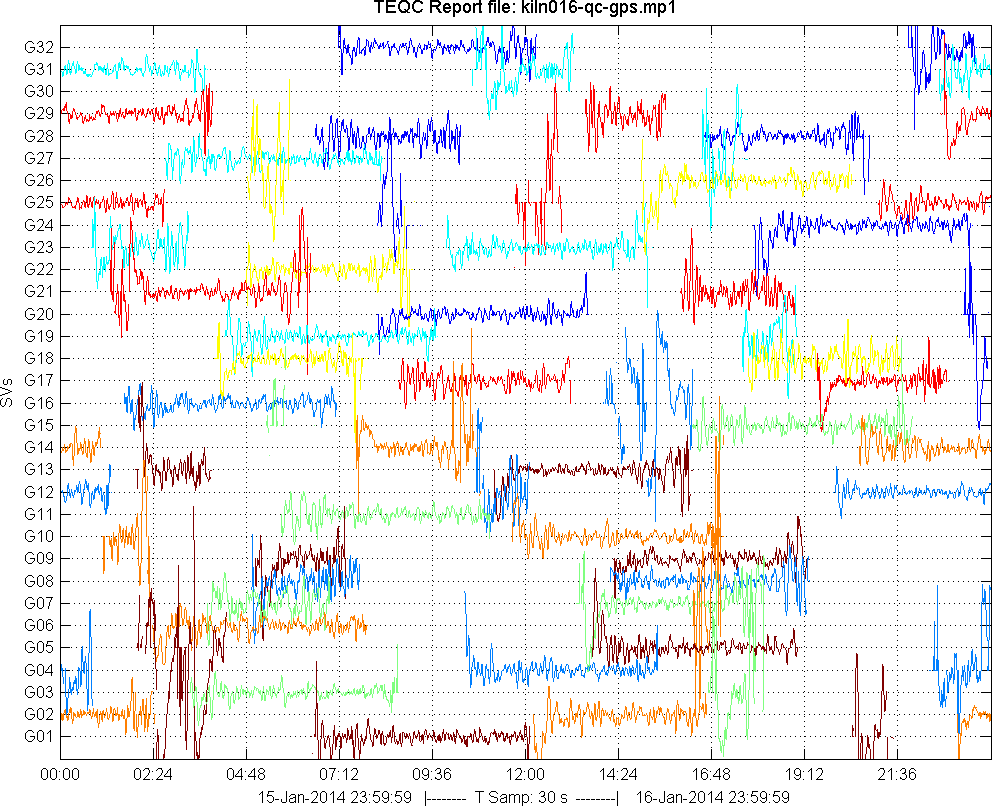
\includegraphics[width=\textwidth]{pic/kiln016_qc_gps_mp1.png}
			\caption{KILN, suspected MP}
			\label{fig:sub2}
		\end{subfigure}
		\caption{Comparison of TEQC MP1 outputs}
		% \label{fig:test}
	\end{figure}
\end{frame}

\begin{frame}{Friday 16/01/15, MP2}
	\begin{figure}
		\centering
		\begin{subfigure}{.5\textwidth}
			\centering
			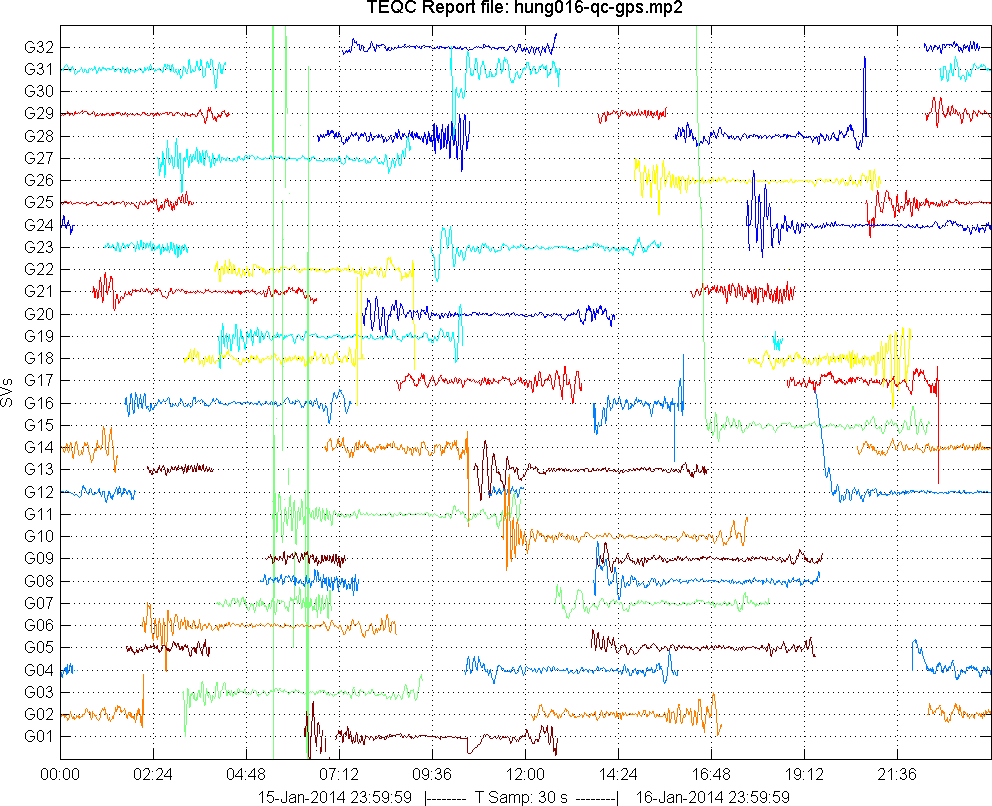
\includegraphics[width=\textwidth]{pic/hung016_qc_gps_mp2.png}
			\caption{HUNG, no MP}
			\label{fig:sub1}
		\end{subfigure}%
		\begin{subfigure}{.5\textwidth}
			\centering
			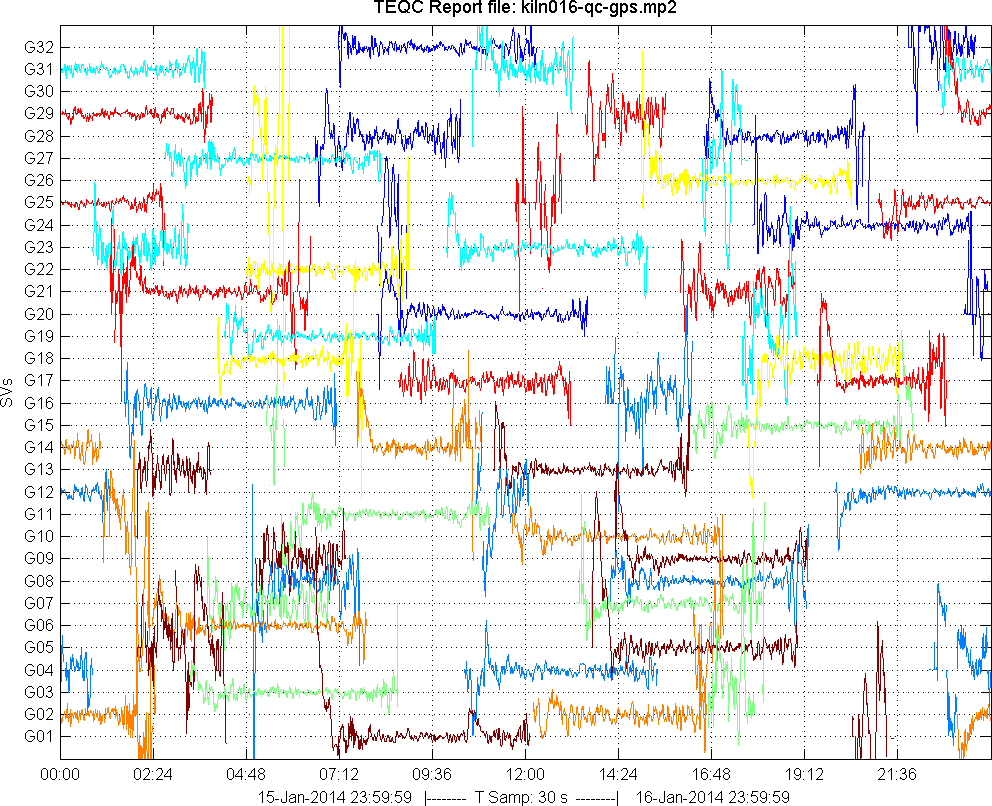
\includegraphics[width=\textwidth]{pic/kiln016_qc_gps_mp2.png}
			\caption{KILN, suspected MP}
			\label{fig:sub2}
		\end{subfigure}
		\caption{Comparison of TEQC MP2 outputs}
		% \label{fig:test}
	\end{figure}
\end{frame}

\begin{frame}{Saturday 17/01/15, MP1}
	\begin{figure}
		\centering
		\begin{subfigure}{.5\textwidth}
			\centering
			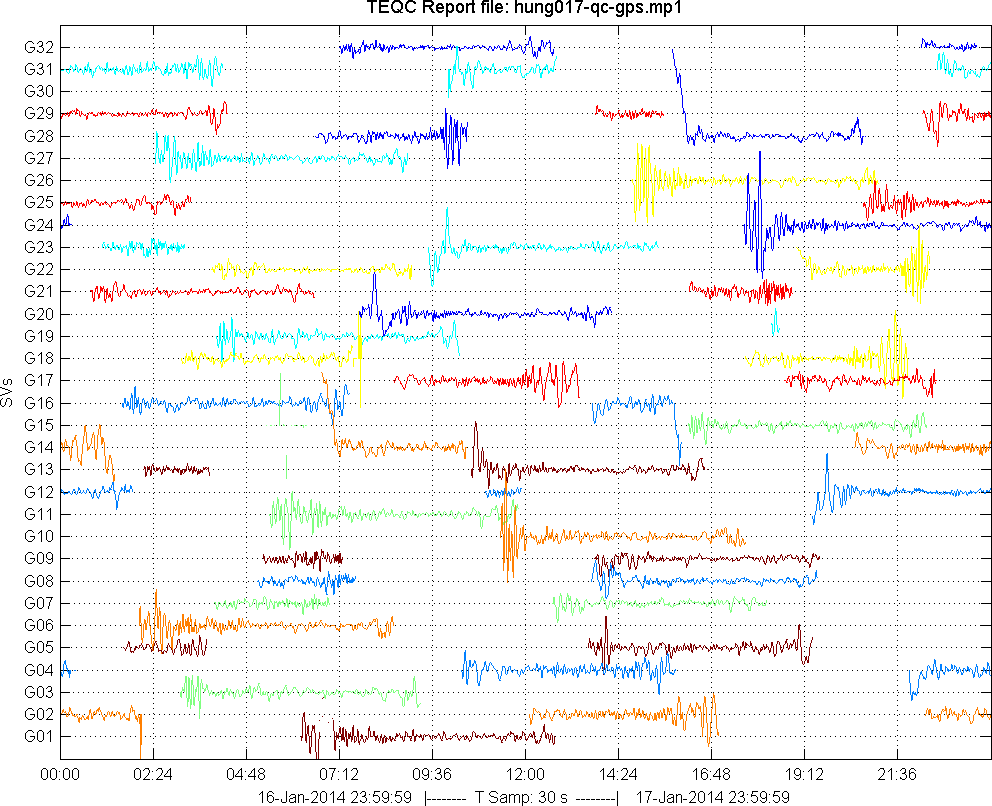
\includegraphics[width=\textwidth]{pic/hung017_qc_gps_mp1.png}
			\caption{HUNG, no MP}
			\label{fig:sub1}
		\end{subfigure}%
		\begin{subfigure}{.5\textwidth}
			\centering
			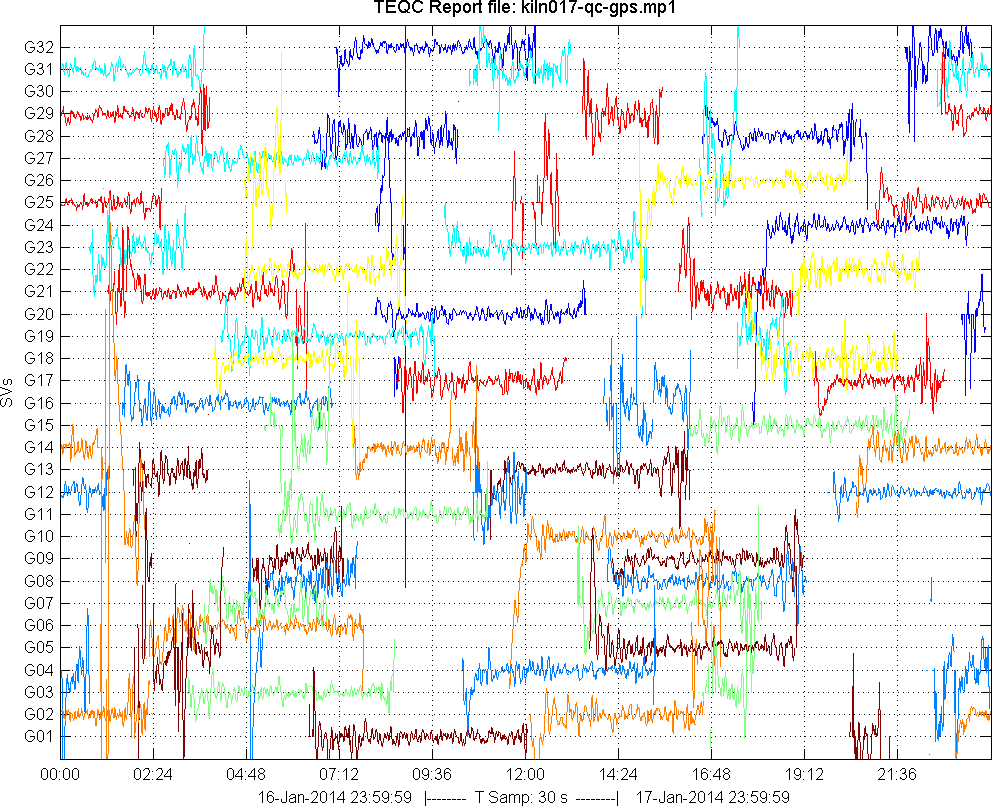
\includegraphics[width=\textwidth]{pic/kiln017_qc_gps_mp1.png}
			\caption{KILN, suspected MP}
			\label{fig:sub2}
		\end{subfigure}
		\caption{Comparison of TEQC MP1 outputs}
		% \label{fig:test}
	\end{figure}
\end{frame}

\begin{frame}{Saturday 17/01/15, MP2}
	\begin{figure}
		\centering
		\begin{subfigure}{.5\textwidth}
			\centering
			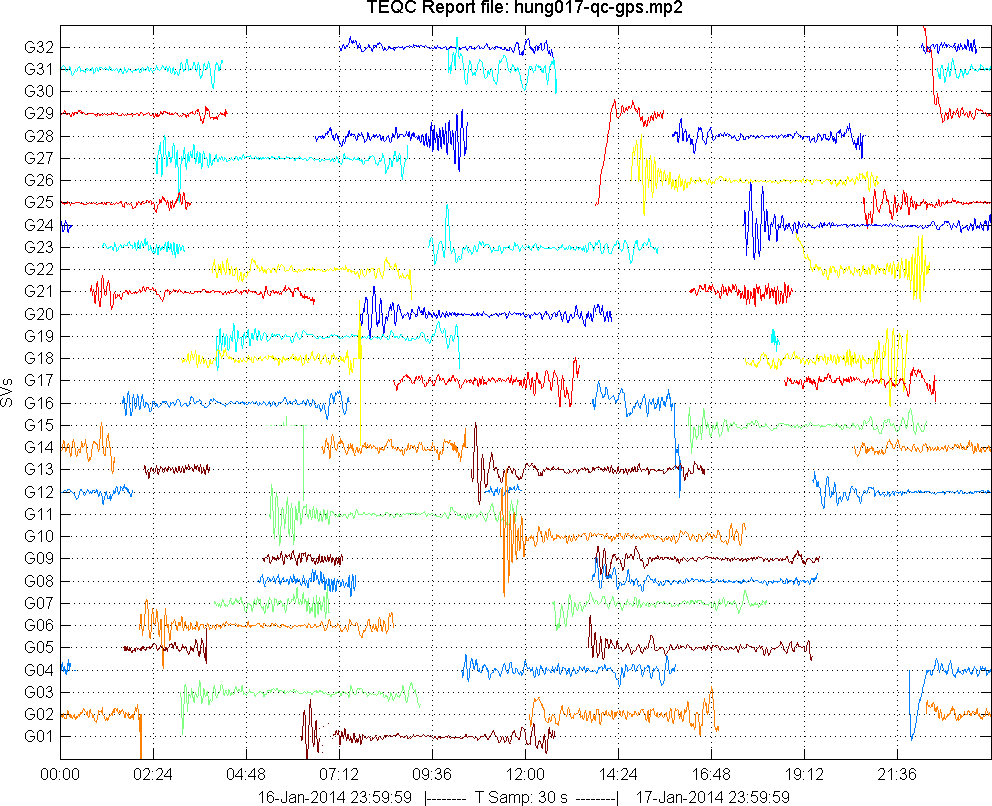
\includegraphics[width=\textwidth]{pic/hung017_qc_gps_mp2.png}
			\caption{HUNG, no MP}
			\label{fig:sub1}
		\end{subfigure}%
		\begin{subfigure}{.5\textwidth}
			\centering
			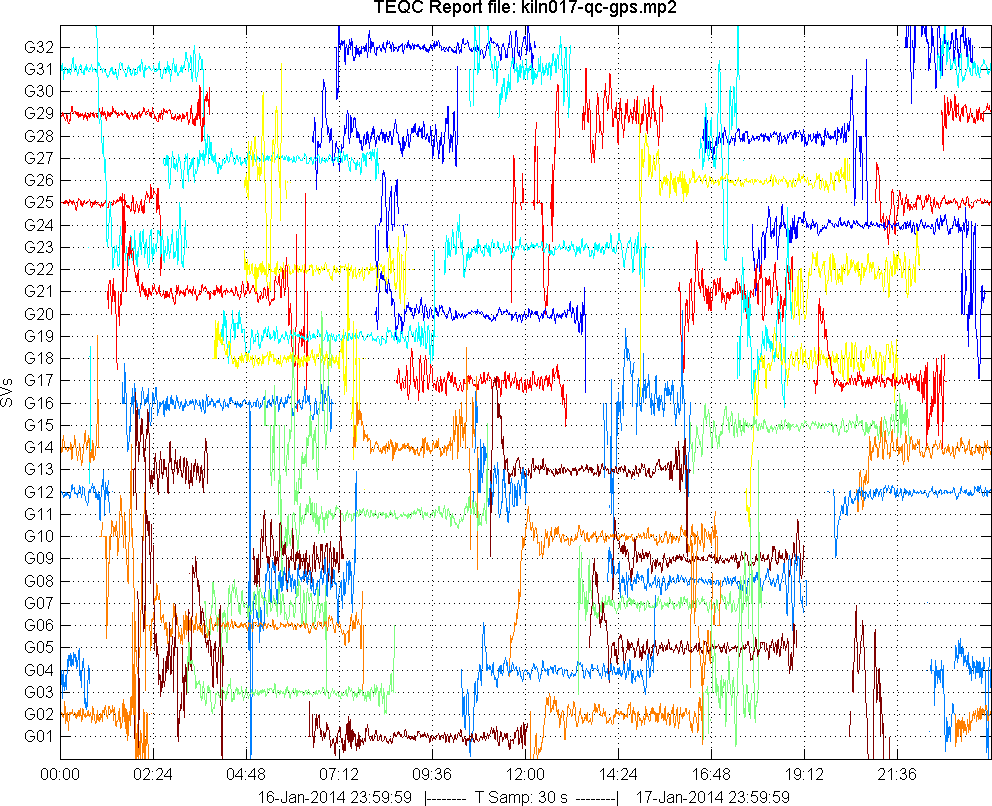
\includegraphics[width=\textwidth]{pic/kiln017_qc_gps_mp2.png}
			\caption{KILN, suspected MP}
			\label{fig:sub2}
		\end{subfigure}
		\caption{Comparison of TEQC MP2 outputs}
		% \label{fig:test}
	\end{figure}
\end{frame}

\begin{frame}{Saturday 17/01/15, MP1}
	\begin{figure}
		\centering
		\begin{subfigure}{.5\textwidth}
			\centering
			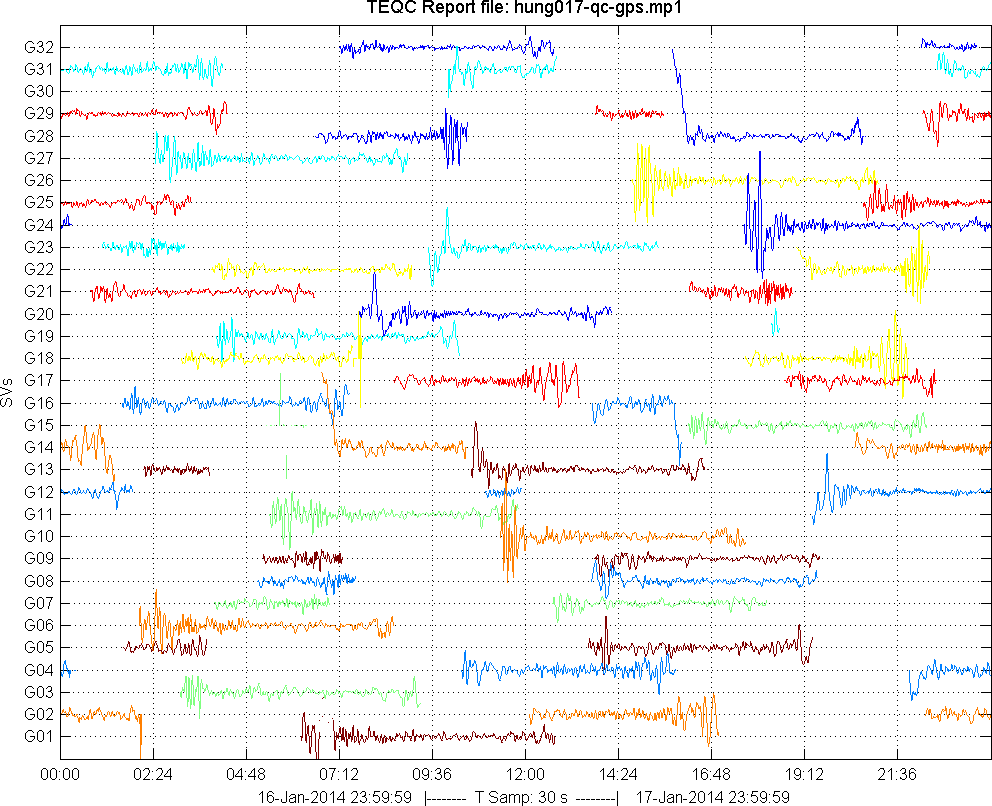
\includegraphics[width=\textwidth]{pic/hung017_qc_gps_mp1.png}
			\caption{HUNG, no MP}
			\label{fig:sub1}
		\end{subfigure}%
		\begin{subfigure}{.5\textwidth}
			\centering
			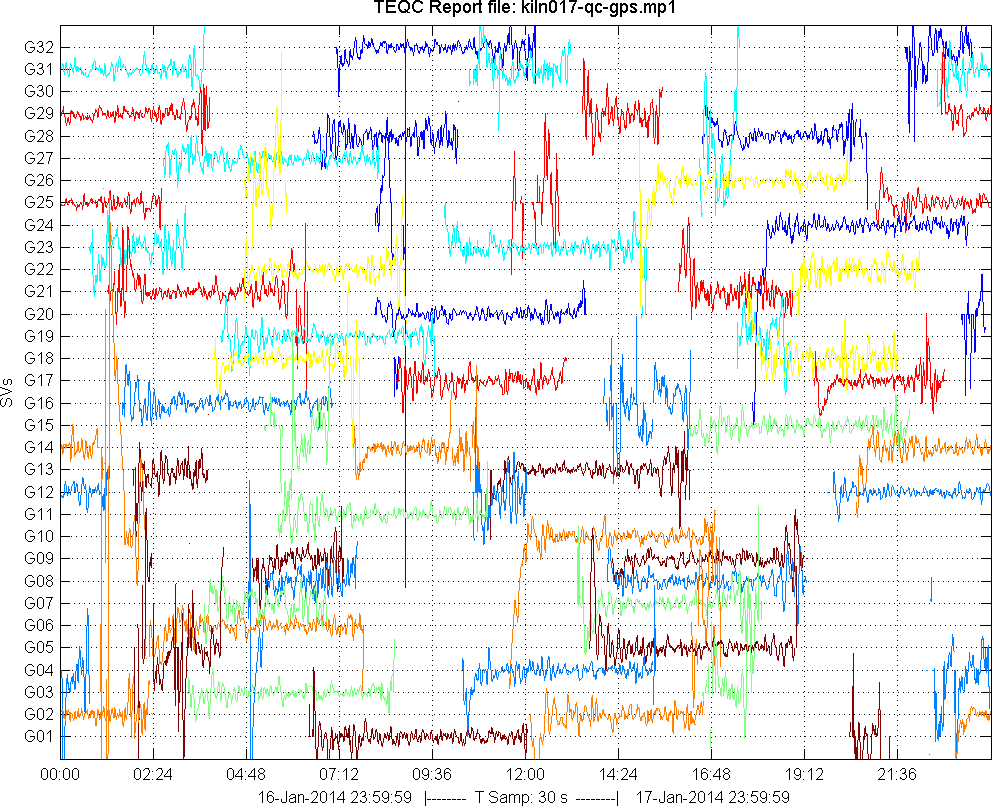
\includegraphics[width=\textwidth]{pic/kiln017_qc_gps_mp1.png}
			\caption{KILN, suspected MP}
			\label{fig:sub2}
		\end{subfigure}
		\caption{Comparison of TEQC MP1 outputs}
		% \label{fig:test}
	\end{figure}
\end{frame}

\begin{frame}{Sunday 18/01/15, MP2}
	\begin{figure}
		\centering
		\begin{subfigure}{.5\textwidth}
			\centering
			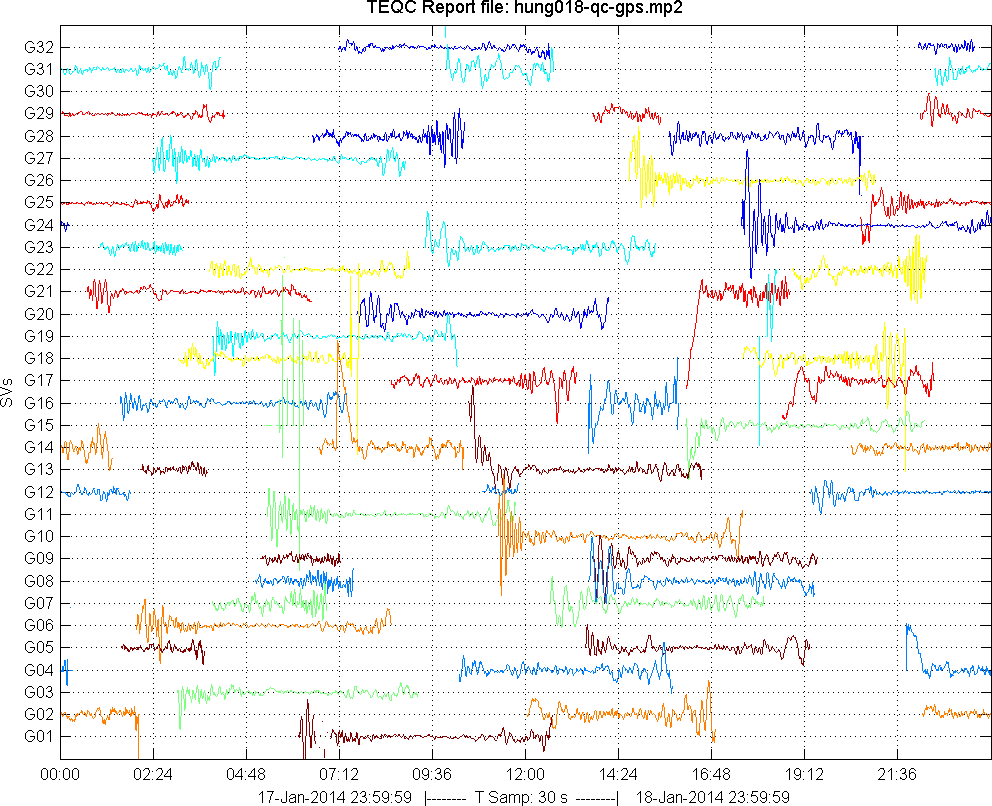
\includegraphics[width=\textwidth]{pic/hung018_qc_gps_mp2.png}
			\caption{HUNG, no MP}
			\label{fig:sub1}
		\end{subfigure}%
		\begin{subfigure}{.5\textwidth}
			\centering
			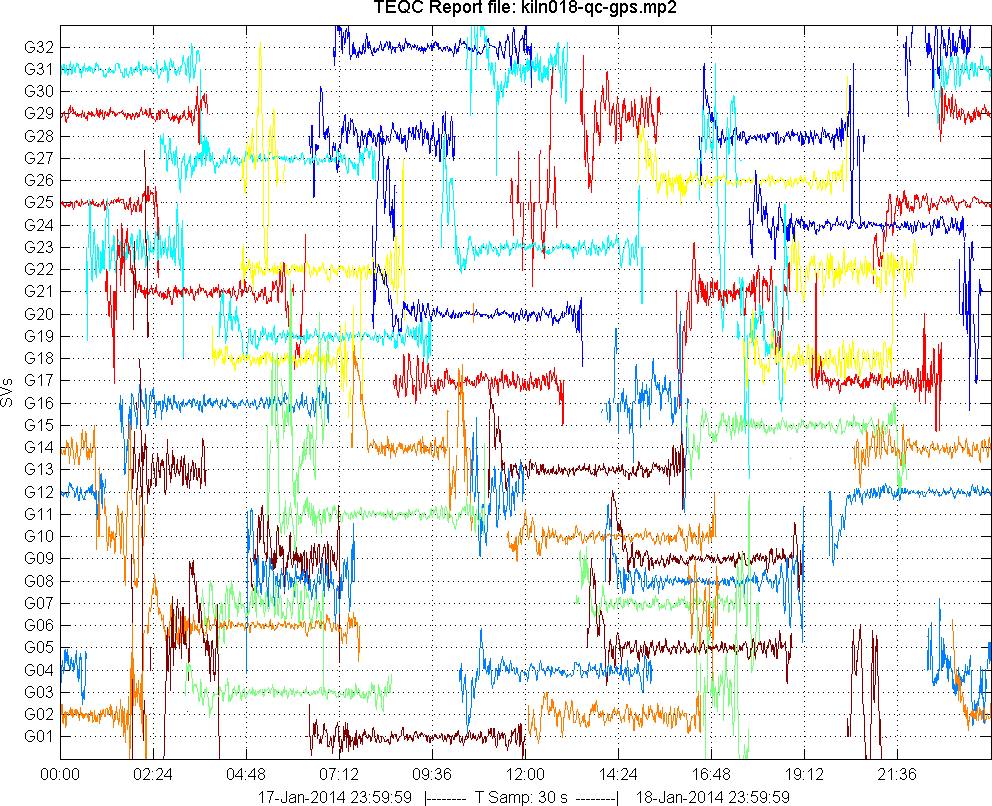
\includegraphics[width=\textwidth]{pic/kiln018_qc_gps_mp2.png}
			\caption{KILN, suspected MP}
			\label{fig:sub2}
		\end{subfigure}
		\caption{Comparison of TEQC MP2 outputs}
		% \label{fig:test}
	\end{figure}
\end{frame}

\begin{frame}{Sunday 18/01/15, MP1}
	\begin{figure}
		\centering
		\begin{subfigure}{.5\textwidth}
			\centering
			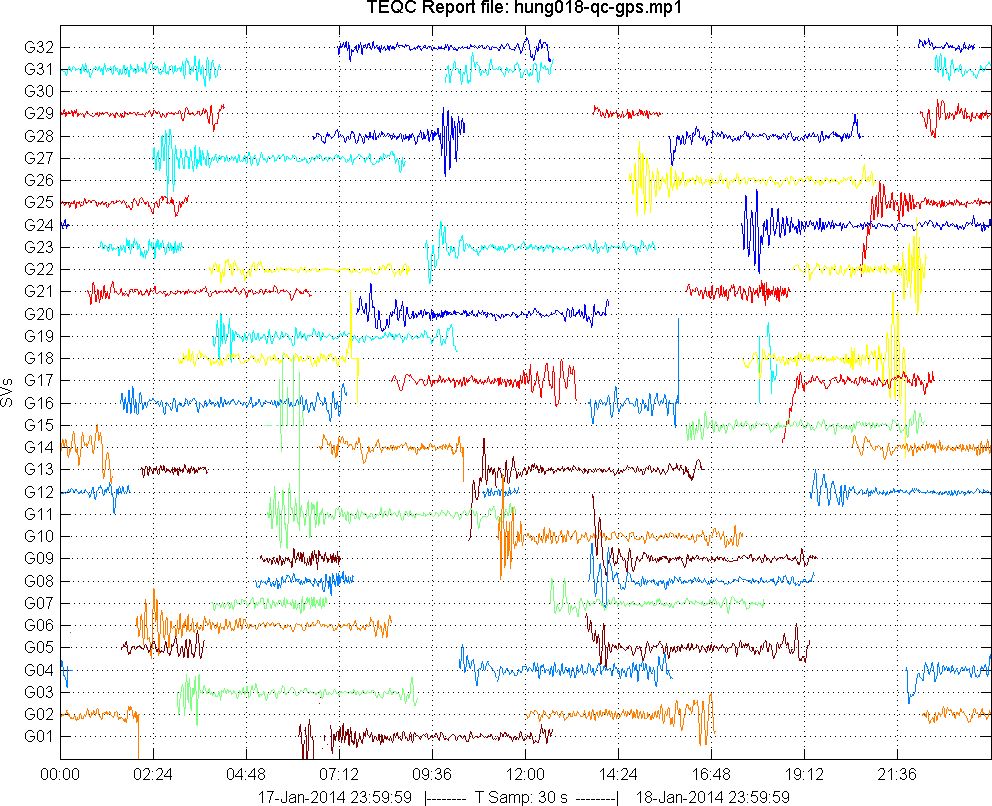
\includegraphics[width=\textwidth]{pic/hung018_qc_gps_mp1.png}
			\caption{HUNG, no MP}
			\label{fig:sub1}
		\end{subfigure}%
		\begin{subfigure}{.5\textwidth}
			\centering
			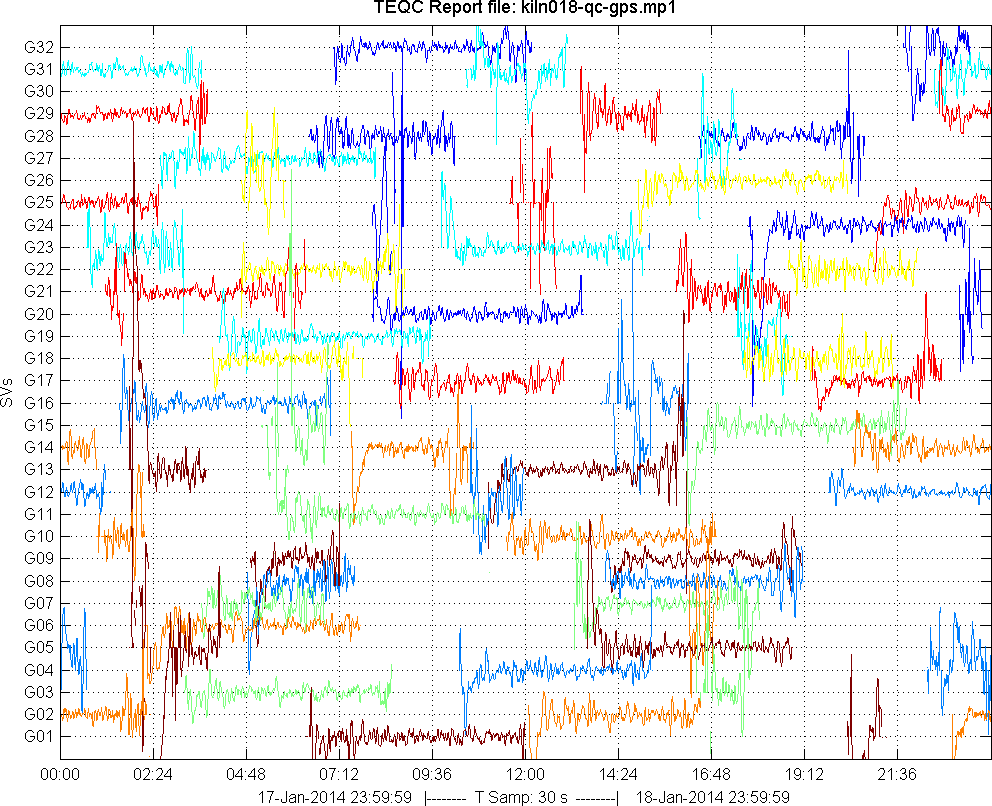
\includegraphics[width=\textwidth]{pic/kiln018_qc_gps_mp1.png}
			\caption{KILN, suspected MP}
			\label{fig:sub2}
		\end{subfigure}
		\caption{Comparison of TEQC MP1 outputs}
		% \label{fig:test}
	\end{figure}
\end{frame}

\begin{frame}{Sunday 18/01/15, MP2}
	\begin{figure}
		\centering
		\begin{subfigure}{.5\textwidth}
			\centering
			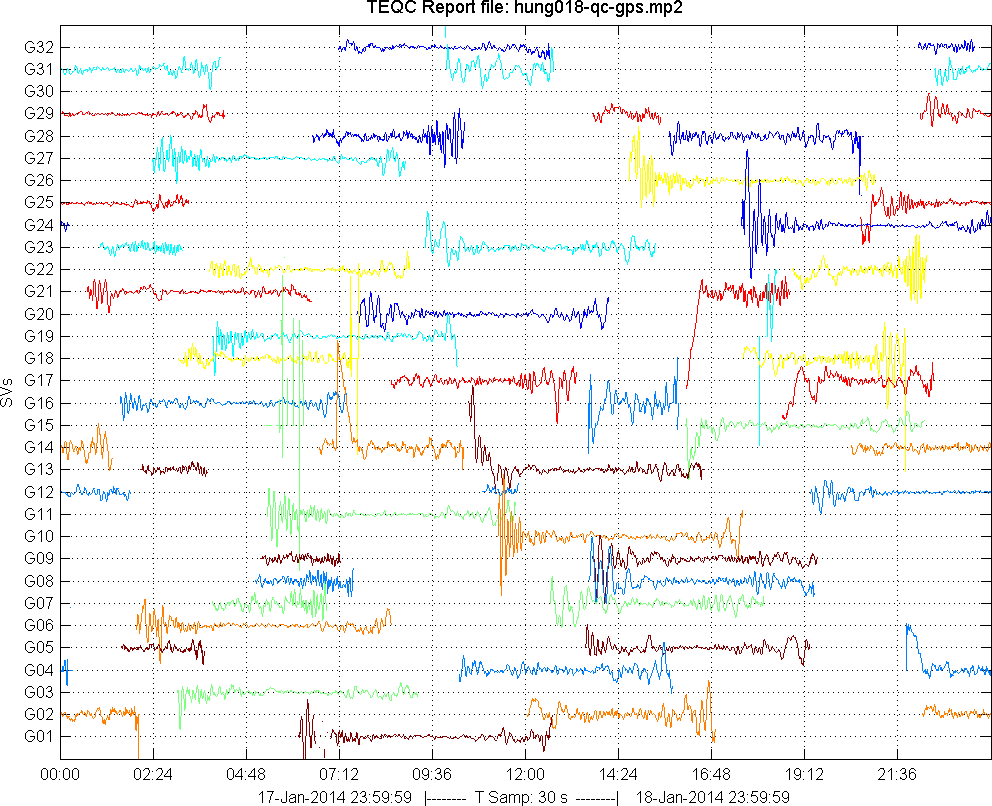
\includegraphics[width=\textwidth]{pic/hung018_qc_gps_mp2.png}
			\caption{HUNG, no MP}
			\label{fig:sub1}
		\end{subfigure}%
		\begin{subfigure}{.5\textwidth}
			\centering
			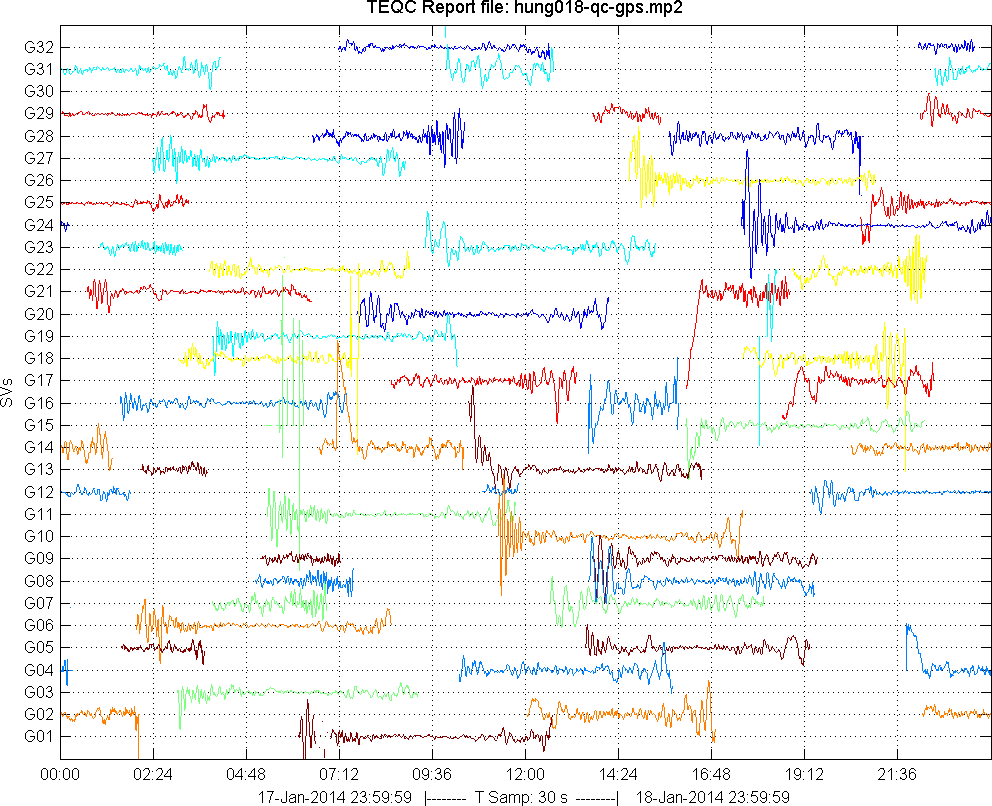
\includegraphics[width=\textwidth]{pic/hung018_qc_gps_mp2.png}
			\caption{KILN, suspected MP}
			\label{fig:sub2}
		\end{subfigure}
		\caption{Comparison of TEQC MP2 outputs}
		% \label{fig:test}
	\end{figure}
\end{frame}	

\begin{frame}{Sunday 18/01/15, MP2}
	\begin{figure}[!htb]
		\centering
		\begin{minipage}{.5\textwidth}
			\centering
			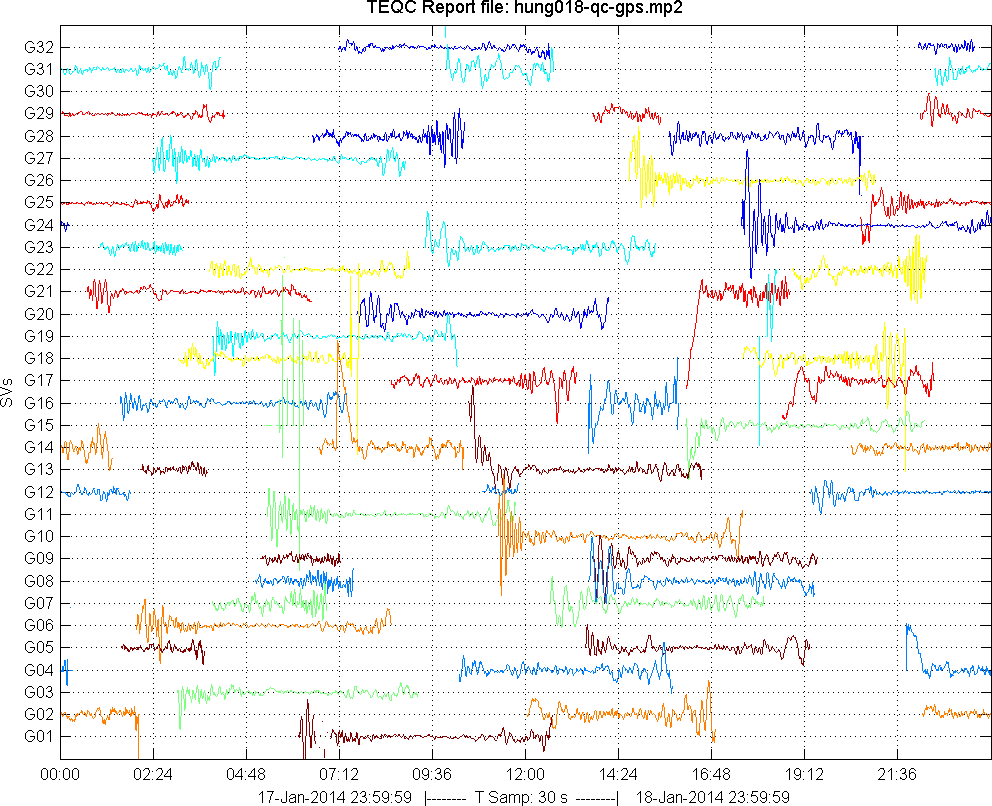
\includegraphics[width=\textwidth]{pic/hung018_qc_gps_mp2.png}
			\caption{$dt=0.1$}
			\label{fig:HUNG, no MP}
		\end{minipage}%
		\begin{minipage}{0.5\textwidth}
			\centering
			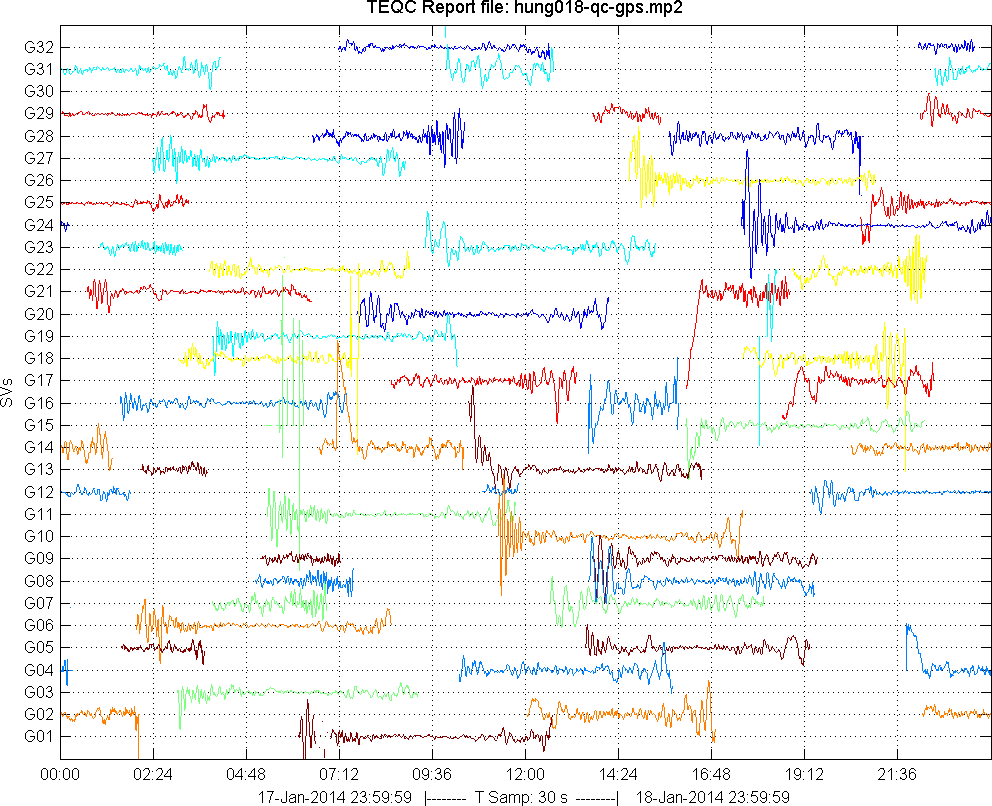
\includegraphics[width=\linewidth]{pic/hung018_qc_gps_mp2.png}
			\caption{$dt =$}
			\label{fig:KILN, suspected MP}
		\end{minipage}
	\end{figure}
\end{frame}	


	%\section{Conclusions}
	
	%\begin{frame}{Conclusions}
	%	\lipsum
	%\end{frame}
	
\end{document}
